\documentclass[11pt,leqno,oneside]{amsart}
\usepackage[alphabetic,abbrev]{amsrefs} % use AMS ref scheme
\usepackage{../ReAdTeX/readtex-core}
\usepackage{../ReAdTeX/readtex-dangerous}
\usepackage{../ReAdTeX/readtex-lie-algebras}
\usepackage{../ReAdTeX/readtex-abstract-algebra}
\usepackage{./monographs}
\usepackage{caption}
\usepackage{subcaption}
\usepackage{todonotes}
\usepackage{tikz-cd}
\numberwithin{thm}{section}

\newcommand{\rootlattice}{\Lambda_R}
\newcommand{\weightlattice}{\Lambda_W}
\newcommand{\halfsum}{\rho}
\renewcommand{\Sym}{S}

\title[Root Systems]{Root Systems}
\author{George H. Seelinger}
\date{February 2017}
\begin{document}
\maketitle
\section{Introduction}
A root system is a configuration of vectors in some Euclidean space
that satisfy nice properties concerning reflections \cite{wiki}. In particular,
root systems are acted upon by associated Weyl groups of
reflections. While root systems have some interesting features in
their own right, they are intimately related to the structure of
semisimple Lie algebras. However, this write-up seeks to simply talk
about what is known about root systems in their own right. A lot of
the definitions and treatments are lifted from \cite{humph} and thus
I do not lay any claim to the originality of statements of
definitions, theorems, etc. I view these notes as mainly a good
companion to be read along with \cite{humph}.
\section{Definitions and Basic Concepts}
Given a vector $\alpha \in E$, we can define a function $\sigma_\alpha \from E
\to E$ that reflects every vector over the hyperplane perpendicular to
$\alpha$. Explicitly, we get \[
  \sigma_\alpha(\beta) = \beta -
  \frac{2(\beta,\alpha)}{(\alpha,\alpha)} \alpha
\]
where $\beta \in E$ and $(\cdot,\cdot)$ is the standard inner product
on $E$. To see this works, note that $\sigma_\alpha(\alpha) = -\alpha$
as desired and if $(\beta,\alpha) = 0$, then $\sigma_\alpha(\beta) =
\beta$, leaving all the vectors in the hyperplane fixed.
\begin{defn}
  For notational convenience, we will say \[
    \langle \beta, \alpha \rangle = \frac{2(\beta,\alpha)}{(\alpha,\alpha)}.
  \]
  It is important to note that $\langle \cdot, \cdot \rangle$ is
  linear only in the first variable.
\end{defn}
\begin{defn}
  \cite{humph}*{p 42} A \de{root system} is a set of vectors $\roots$ in
  Euclidean space $E$
  such that
  \begin{itemize}
  \item $\roots$ is finite, $\Span \roots = E$, and $0 \not \in \roots$.
  \item If $\alpha \in \roots$, then the only multiples of $\alpha$ in
    $\roots$ are $\pm \alpha$.
  \item If $\alpha \in \roots$, then $\sigma_\alpha(\roots) = \roots$
  \item If $\alpha,\beta \in \roots$, then $\langle  \beta,\alpha
    \rangle \in \Z$.
  \end{itemize}
\end{defn}
\begin{example}
  Consider the collection of vectors in $\R^2$ of equal length with
  angle from 
  the origin given in multiples of 60 degress. Such a collection is a
  root system, as can be easily checked.
  \begin{figure}[h]
    \centering
    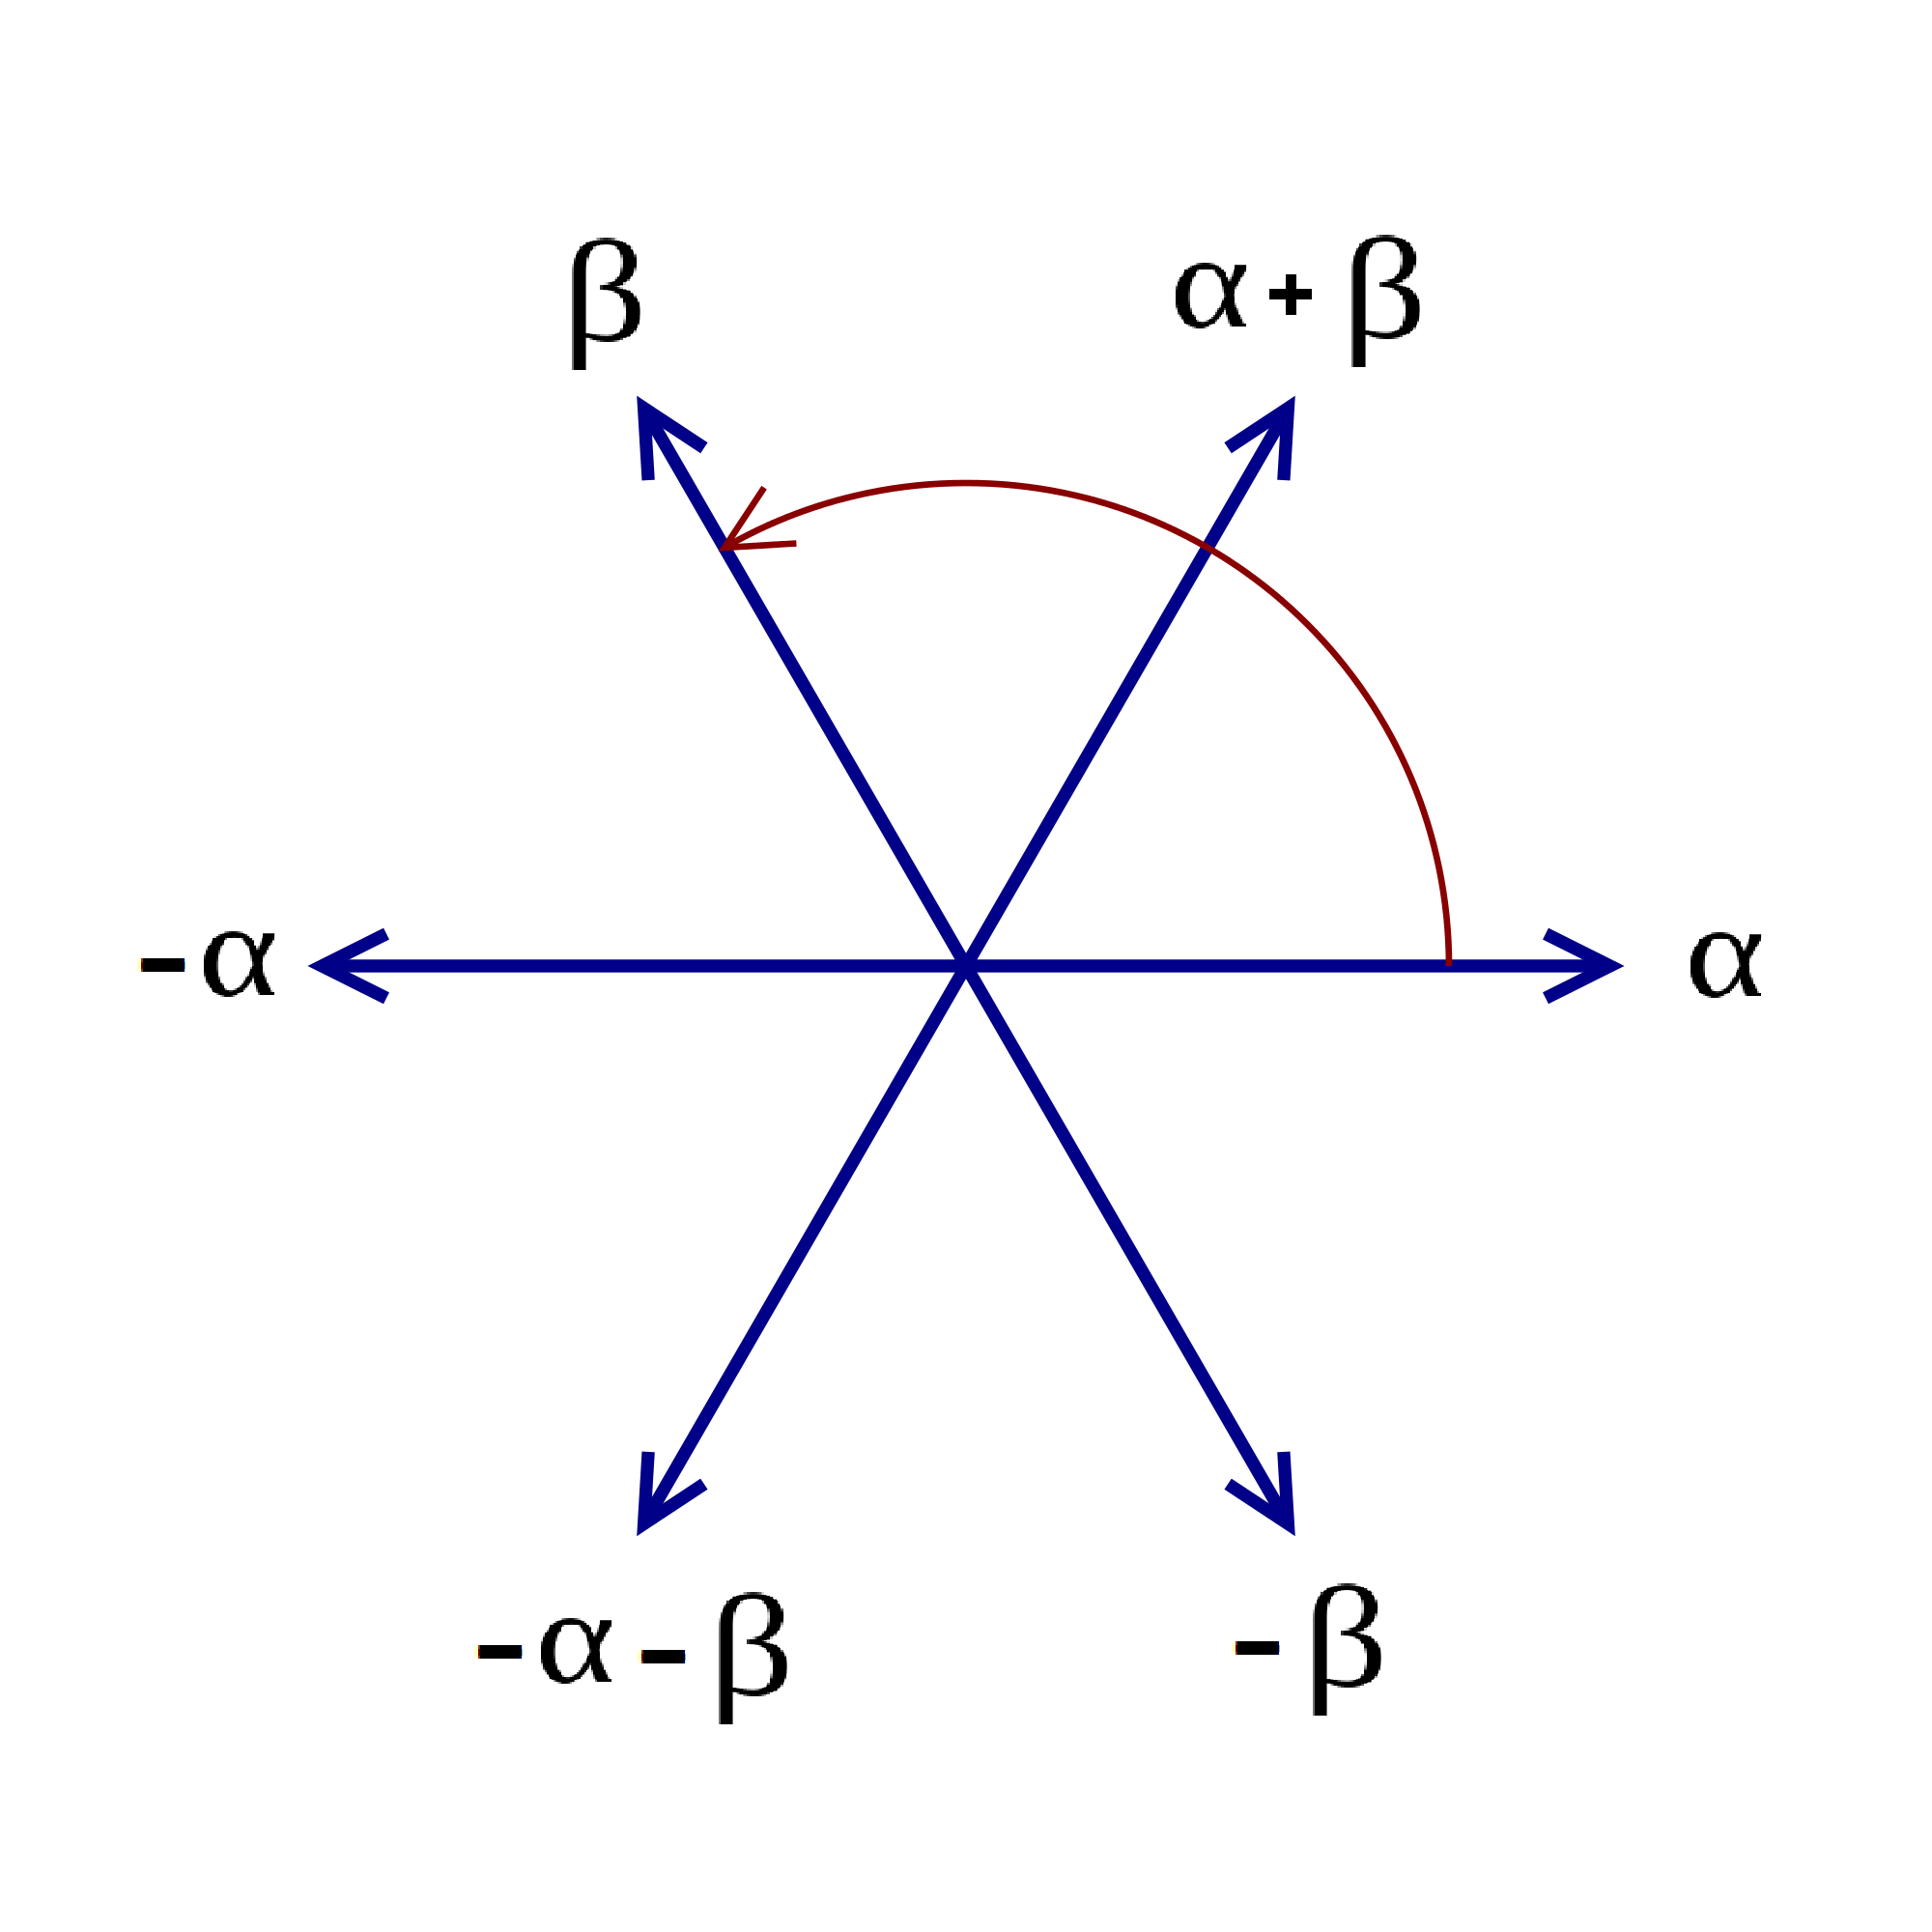
\includegraphics[width=0.25\textwidth]{images/Root_system_A2_with_labels.png}
    \caption{Root system $A_2$ from \cite{wiki}}
  \end{figure}
\end{example}
These hyperplane reflections form a ``nice''
action of the root system. Furthermore, 
they generate a group, since the composition of two reflections will
still map root vectors of a root system to root vectors and each reflection is invertible.
\begin{defn}
  The \de{Weyl group} of a root system is the collection of these
  reflections $\sigma_\alpha$ with group operation as
  composition. Explicitly, \[
    \W = \langle \{\sigma_\alpha \mid \forall \alpha \in \roots\} \mid
    \{\sigma_\alpha^2 = 1, \ \forall \alpha \in \roots\} \rangle
  \]
\end{defn}
It is a straightfoward exercise to show the following fact
\begin{lem}\label{weyl-gp-conj}
  \cite{humph}*{p 43} If $\sigma \in GL(E)$ leaves \(\roots\) invariant and $\sigma_\alpha \in
  \W$ is a simple reflection, then \[
    \sigma \sigma_\alpha \sigma^{-1} = \sigma_{\sigma(\alpha)}
  \]
  and also \[
    \langle \sigma(\beta), \sigma(\alpha) \rangle = \langle \beta, \alpha \rangle
  \]
\end{lem}
\begin{defn}
  We say a root system is \de{reducible} if there exists root systems
  \(\roots_1, \roots_2 \subset \roots\) such that \(\roots = \roots_1 \dunion
  \roots_2\) such that \(\Span(\roots) = \Span(\roots_1) \oplus
  \Span(\roots_2)\). Any root system that is not reducible is called
  \de{irreducible}. 
\end{defn}
In general, we restrict our attention to irreducible root systems,
since they are the basic building blocks of root systems.
Now, we also have a convenience of notation as follows
\begin{defn}
   For $\alpha \in \roots$, a root system, we say a \de{coroot}
   $\alpha^\vee$ is given by \[ 
    \alpha^\vee = \frac{2 \alpha}{(\alpha, \alpha)}
  \]
\end{defn}
It is worth noting that $\roots^\vee$ is also a root system with an
associated Weyl group that is isomorphic to the Weyl group of $\roots$.
\begin{defn}
  We define the \de{rank} of a root system $\roots$ to be the dimension
  of Euclidean space it spans.
\end{defn}
The axioms for a root system are fairly restrictive, and so it is
relatively easy to classify all the possible root systems that span
$\R$ and $\R^2$. Namely, since \((\alpha,\beta) =
\norm[\alpha]\norm[\beta] \cos \theta\), \[
  \langle \alpha,\beta \rangle \langle \beta,\alpha \rangle = 4 \cos^2
  \theta \in \Z_{\geq 0}
\]
Thus, we have the following
\begin{lem}\label{possible-values-of-inner-product}
  Let \(\alpha,\beta \in \roots\) with \(\beta \neq \pm \alpha\),
  then \[ 
    \langle \alpha,\beta \rangle \langle \beta,\alpha \rangle \in \{0,1,2,3\}
  \]
\end{lem}
\begin{proof}
  This follows immediately from \(\langle \alpha,\beta \rangle\) and
  \(\langle \beta,\alpha \rangle\) being integers and \(4 \cos^2
  \theta \leq 4\).
\end{proof}
Thus, roots can only ever have certain angles
between them. To see this, examine Table 1 on page 45 of
\cite{humph}. 

However, these restrictions lead us to a useful
application for determining when sums and differences of roots are
roots.
\begin{lem}
  \cite{humph}*{p 45} Let $\alpha,\beta \in \roots$ be nonproportional
  roots.
  \begin{itemize}
  \item If $(\alpha,\beta) > 0$, then $\alpha-\beta \in \roots$.
  \item If $(\alpha,\beta) < 0$, then $\alpha+\beta \in \roots$.
  \end{itemize}
\end{lem}
\begin{proof}
  Note \((\alpha,\beta) > 0 \iff \langle \alpha,\beta \rangle >
  0\). By the table of values, the acuteness of the angle requires
  that either \(\langle \alpha,\beta \rangle\) or \(\langle
  \beta,\alpha \rangle\) is \(1\). Thus, by the axioms of the root
  system, \(\langle \alpha,\beta \rangle = 1 \implies
  \sigma_\beta(\alpha) = \alpha-\beta \in \roots\) or \(\langle
  \beta,\alpha \rangle = 1 \implies \beta-\alpha \in \roots \implies
  \alpha-\beta \in \roots\).
\end{proof}
An application of this lemma is to justify the existence of
unbroken ``strings'' of roots of the form $\beta + n \alpha, n \in \Z,
q \leq n \leq r$. \todo{Write this in more formally.}
\begin{defn}
  \cite{humph}*{p 47} Given $\simpleroots \subset \roots$, we say that $\simpleroots$ is a \de{simple
    system} or \de{base} if
  \begin{itemize}
  \item $\simpleroots$ is a basis for $\Span \roots$
  \item Every $\beta \in \roots$ can be written as $\beta = \sum
    k_\alpha \alpha$ with $\alpha \in \simpleroots$ and all $k_\alpha \in
    \Z_{\geq 0}$ or all $k_\alpha \in \Z_{\leq 0}$.
  \end{itemize}
\end{defn}
We note that $\simpleroots$ need not be unique and so whenever any
definition depends on $\simpleroots$, there is a choice being made that must
be accounted for.
\begin{defn}
  The \de{height} of $\beta \in \roots$ relative to $\simpleroots$ is given
  by \[
    \operatorname{ht}(\beta) = \sum_{\alpha \in \simpleroots} k_\alpha
  \]
  where $\beta = \sum_{\alpha \in \simpleroots} k_\alpha \alpha$. 
\end{defn}
Using this notion of height, we can define positive roots
relative to $\simpleroots$ as those with $k_\alpha \geq 0, \forall \alpha
\in \simpleroots$ and a similar notion for negative roots. Note that this
partitions $\roots = \roots^+ \dunion \roots^-$. We also note that we can
define a partial order on the roots in $\roots$ with a fixed $\simpleroots$.
\begin{defn}\label{partial-order-on-roots}
  \cite{humph}*{p 47} We say $\mu \prec \lambda$ if and only if $\lambda - \mu$ is a sum
  of positive roots (equivalently, of simple roots) or $\lambda =
  \mu$. 
\end{defn}
We note also the following relationship between simple roots.
\begin{lem}\label{a-b-not-a-root}
  \cite{humph}*{p 47} If $\simpleroots$ is a base of $\roots$, then $(\alpha,
  \beta) \leq 0$ for $\alpha \neq \beta$ in $\simpleroots$, and $\alpha -
  \beta$ is not a root.
\end{lem}
\begin{proof}
  For \(\alpha,\beta \in \simpleroots\), let \((\alpha,\beta) >
  0\). Then, \(\alpha-\beta \in \roots\), which violates the second
  axiom of a base. 
\end{proof}
In essence,
this lemma gives us that the angle between two simple roots is obtuse.
\begin{defn}\label{half-sum-defn}
  Let us define the \de{half sum of positive roots} as \[
    \halfsum := \frac{1}{2}
  \sum_{\beta \succ 0} \beta.
\]
\end{defn}
This vector (not necessarily a root) has some important properties,
such as the following
\begin{prop}
  \cite{humph}*{p 50} $\sigma_\alpha(\halfsum) = \halfsum-\alpha$ for all
  $\alpha \in \simpleroots$.
\end{prop}
Now, we wish to show the following existence theorem.
\begin{thm}
  Every root system has a base.
\end{thm}
To do this, we will make use of the fact
\begin{prop}
  The union of finitely many hyperplanes cannot be all of \(\R^n\) for
  \(n \geq 2\).
\end{prop}
As a result of this proposition, we may choose a vector in our
Euclidean space \(E\) which does not lie in any hyperplane
perpendicular to a root.
\begin{defn}
  We call a vector \(z \in E\) \de{regular} if \(z \in E \setminus
  \Union_{\alpha \in \roots} P_\alpha\), where \(P_\alpha\) is the
  hyperplane orthogonal to the root \(\alpha\), and \de{singular} otherwise.
\end{defn}
\begin{defn}
  Given a vector \(z \in E\), we define \[
    \roots^+(z) := \{\alpha \in \roots \st (z,\alpha) > 0\}
  \]
  We also say \(\alpha \in \roots^+(z)\) is \de{decomposable} if
  \(\alpha = \beta_1 + \beta_2\)  for some \(\beta_i \in
  \roots^+(z)\). Otherwise, it is \de{indecomposable}.
\end{defn}
\begin{prop}
  If \(z \in E\) is regular, then \[
    \roots = \roots^+(z) \union \roots^+(-z)
  \]
\end{prop}
Thus, following \cite{humph}, we rewrite our theorem above in a more
explicit manner.
\begin{thm}\label{regular-vec-and-base}
  Let \(z \in E\) be regular. Then, the set \(\simpleroots(z)\) of all
  indecomposable 
  roots in \(\roots^+(z)\) is a base of \(\roots\) and every base of
  \(\roots\) has the form \(\simpleroots(z')\) for some regular \(z'
  \in E\).
\end{thm}
\begin{proof}
  Let \(\dim E \geq 2\), otherwise the theorem is immediate. Now,\(\beta
  \in \roots \implies \beta \in \roots^+(z)\) or \(-\beta \in 
  \roots^+(z)\) by the proposition above, so we need only show \[
    \beta = \sum_{\alpha \in \simpleroots^+(z)} k_\alpha \alpha, \
    k_\alpha \in \Z_{\geq 0}
  \]
  Assume that is not the case. Then, we may pick a \(\beta \in
  \roots^+(z)\) such that \((z,\beta)\) is as small as possible. Since
  \(\beta \not \in \simpleroots(z)\), there is a \(\beta_1, \beta_2
  \in \roots^+(z)\) such that \[
    \beta = \beta_1 + \beta_2 \implies (z,\beta) = (z,\beta_1) +
    (z,\beta_2) > 0
  \]
  but then either \(\beta_1\) or \(\beta_2\) is not a positive
  integral linear combination of elements in \(\simpleroots(z)\),
  contradicting \(\beta_i \in \roots^+(z)\).

  Now, we need only show the elements of \(\simpleroots(z)\) are
  linearly independent. By the lemma \ref{a-b-not-a-root}, \((\alpha,\beta) \leq 0\)
  for \(\alpha,\beta \in \simpleroots(z)\) with \(\beta \neq \pm
  \alpha\). Thus, for \(c_\alpha \in \R\), 
  \begin{align*}
    \sum_{\alpha \in \simpleroots(z)} c_\alpha \alpha = 0
    & \implies x := \sum_{\alpha \st r_\alpha > 0} r_\alpha \alpha =
      \sum_{\beta \st r_\beta < 0 } (-r_\beta) \beta \\
    & \implies (x,x) = \sum_{\substack{\alpha \st r_\alpha > 0 \\
    \beta \st r_\beta < 0}} -r_\alpha r_\beta (\alpha,\beta) \leq 0 \\
    & \implies x = 0 \\
    & \implies 0 = (x,z) = \sum_{\alpha \st r_\alpha > 0} r_\alpha
      \cdot (\alpha, z)
  \end{align*}
  where \((\alpha,z) > 0\) since \(\alpha \in \roots^+(z)\) by
  definition, so it must be that all the \(r_\alpha = 0\) and
  similarly for all \(r_\beta\), thus giving linear independence. \\

  Thus, \(\simpleroots(z)\) is a base of \(\roots = \roots^+(z) \union
  \roots^+(-z)\) since \(\simpleroots(z)\) spans \(\roots^+(z)\) and
  thus all of \(\roots\), and it meets the base axioms by above. \\

  To show every base of \(\roots\) has the form \(\simpleroots(z)\)
  for some regular \(z \in E\), we start with a given base
  \(\simpleroots\) and pick a \(z \in E\) so that \((z,\alpha) > 0\)
  for all \(\alpha \in \simpleroots\), which is possible since the
  intersection of the positive open half-spaces associated with any basis
  will be non-empty. Thus, \(z\) is regular, \(\roots^+ \subset
  \roots^+(z)\), and \(\roots^- \subset \roots^+(-z)\), so \(\roots^+
  = \roots^+(z)\). Since \(\simpleroots\) contains only indecomposable
  elements, \(\simpleroots \subset \simpleroots(z)\), but
  \(|\simpleroots| = |\simpleroots(z)| = \ell \implies \simpleroots =
  \simpleroots(z)\). 
\end{proof}
\begin{rmk}
  In plain geometric language, the linear independence argument in the
  above proof shows that any set of
  vectors lying strictly on one 
  side of a hyperplane in Euclidean space and forming pairwise obstuse
  angles must be linearly independent.
\end{rmk}
\section{Standard Examples}\label{standard-examples}
Above, we saw the root system \(A_2\). Classically, some standard
 root systems are of types \(A_n, B_n, C_n\), and
\(D_n\), all of rank \(n\). Whe \(n=2\), each of these has simple system \(\simpleroots =
\{\alpha,\beta\}\), which is suggestively given by the labeling in the diagrams.
\begin{figure}
  \begin{subfigure}{.3\textwidth}
    \centering
    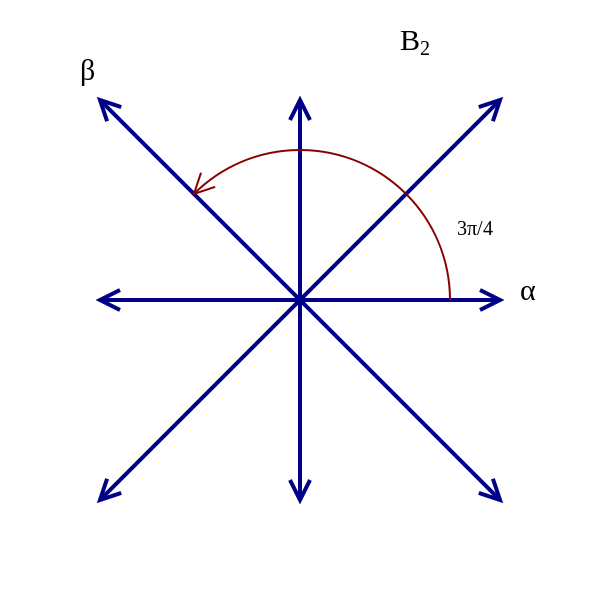
\includegraphics[width=\textwidth]{images/Root_system_B2_with_labels.png}
    \caption{Root system $B_2$}
  \end{subfigure}
  \begin{subfigure}{.3\textwidth}
    \centering
    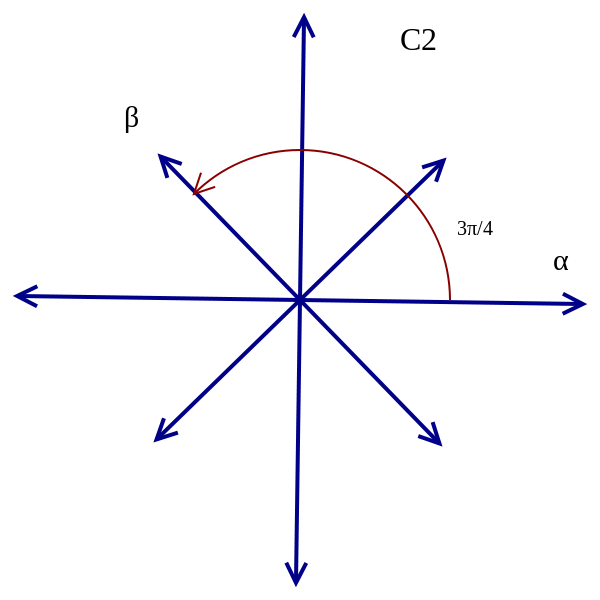
\includegraphics[width=\textwidth]{images/Root_system_C2_with_labels.png}
    \caption{Root system $C_2$}
  \end{subfigure}
  \begin{subfigure}{.3\textwidth}
    \centering
    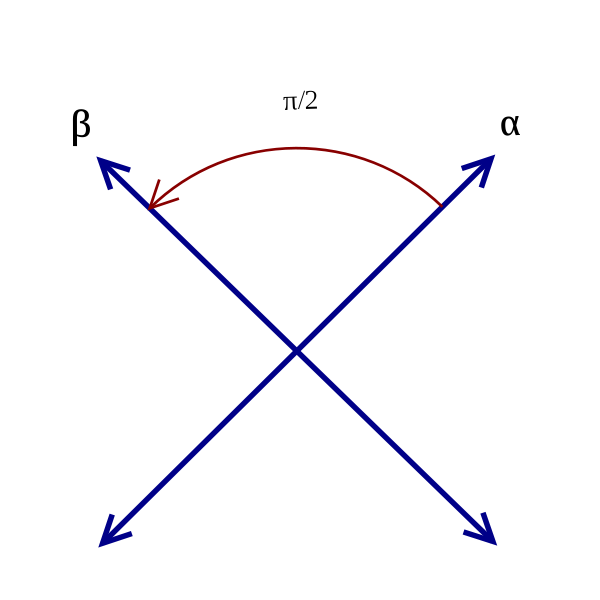
\includegraphics[width=\textwidth]{images/Root_system_D2_with_labels.png}
    \caption{Root system $D_2$ (not irreducible.)}
  \end{subfigure}
  \caption{Classical irreducible root systems when \(n=2\) from \cite{wiki}}
\end{figure}
Note that in \(B_2\), \(|\beta| = \sqrt{2} |\alpha|\) and in \(C_2\),
\(|\alpha| = \sqrt{2}|\beta|\). More formally, we define these systems
for any \(n \in \N\).
\begin{defn}
  Let \(V\) be the subspace of \(\R^{n+1}\) for which the coordinates
  sum to \(0\) and let \(\roots\) be the set of vectors in \(V\) that
  have length \(\sqrt{2}\) and integer coordinates in
  \(\R^{n+1}\). We call \(\roots\) the
  \de{\(A_n\) root system}.
\end{defn}
\begin{defn}
  Let \(\roots\) be all integers in \(\R^n\) having length \(1\) or
  \(\sqrt{2}\) and integer coordinates. We call \(\roots\) the
  \de{\(B_n\) root system}.
\end{defn}
\begin{defn}
  Let \(\roots\) be all vectors in \(\R^n\) having length
  \(\sqrt{2}\) and integer coordinates, as well as all vectors \(2v\)
  where \(v\) is vector having 
  length \(1\) and integer coordinates. Then, we call \(\roots\)
  the \de{\(C_n\) root system}.
\end{defn}
\begin{defn}
  Let \(\roots\) be all vectors in \(\R^n\) having length \(\sqrt{2}\)
  and integer coordinates. We call \(\roots\) the \de{\(D_n\) root
    system}.
\end{defn}
It turns out that all these root systems are irreducible, but they are
not the only ones. There are other so-called ``exceptional'' types,
such as
\begin{defn}
  The following configuration of roots in figure \ref{fig:G_2} is called \(G_2\). \\
  \begin{figure}
  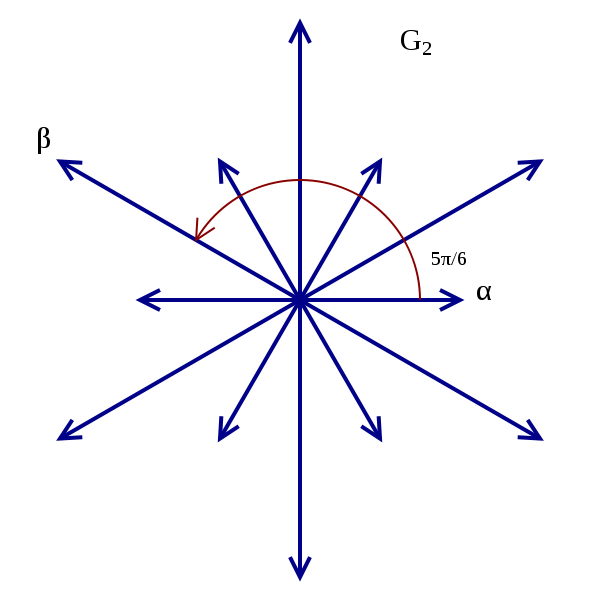
\includegraphics[scale=0.3]{images/Root_system_G2_with_labels}    
    \caption{\(G_2\) Root System from \cite{wiki}}
    \label{fig:G_2}
  \end{figure}
\end{defn}
\begin{rmk}
  Note that the short roots in \(G_2\) form the system \(A_2\), and
  similarly for the long roots.
\end{rmk}
Using Dynkin diagrams, we will arrive at \emph{all}
the irreducible root systems. While it might take a little work to
derive directly at this stage, the root systems
have the following Weyl groups, presented in Table
\ref{tab:wely-groups}, which we will derive later. \\
\begin{table}
  \centering
  \begin{tabular}{|c|c|}
  \hline \(A_n\) & \(S_{n+1}\) \\
  \hline \(B_n\) & \((\Z/2)^n \rtimes S_n\) \\
  \hline \(C_n\) & \((\Z/2)^n \rtimes S_n\)\\
  \hline \(D_n\) & \((\Z/2)^{n-1} \rtimes S_n\) \\
  \hline \(G_2\) & \(D_{12}\), the Dihedral group of order \(12\). \\
  \hline
  \end{tabular}
  \caption{Weyl Groups for Standard Irreducible Root Systems}
  \label{tab:wely-groups}
\end{table}
% We also note, for \(n=2\), the positive systems of \(A_2, B_2, C_2\) are given by the
% roots with positive height. So, for \(A_2\), these are \(\alpha,
% \alpha+\beta,\beta\). 
% In general, if we label our simple system by
% \(\simpleroots = \{\epsilon_1, \ldots, \epsilon_n\}\) this gives us the following values
% for \(\halfsum\). \\
% \begin{tabular}{|c|c|}
%   \hline \(A_n\) & \(\epsilon_1 + \cdots + \epsilon_n\) \\
% z  
% \end{tabular} \\
\section{Weyl Groups}
Weyl groups have some interesting and useful properties as
groups. Furthermore, an arbitrary Weyl group may have group actions on
sets of ``weights'' (discussed later), not just root systems. \\

We start with a useful theorem for how Weyl groups interact with root
systems and their bases
\begin{thm}\label{weyl-gp-and-simple-system}
  \cite{humph}*{Thm 10.3} Let \(\simpleroots\) be a base of \(\roots\).
  \begin{enumerate}
  \item If \(z \in E\) is regular, then there exists \(\sigma \in \W\)
    such that \((\sigma(z), \alpha) > 0\) for all \(\alpha \in
    \simpleroots\).
  \item If \(\simpleroots'\) is another base of \(\roots\), then
    \(\sigma(\simpleroots') = \simpleroots\) for some \(\sigma \in
    \W\). In other words, \(\W\) acts transitively on bases.
  \item If \(\alpha \in \roots\), there exists \(\sigma \in \W\) such
    that \(\sigma(\alpha) \in \simpleroots\)
  \item \(\W\) is generated by \(\{\sigma_\alpha \st \alpha \in
    \simpleroots\}\). 
  \item If \(\sigma(\simpleroots) = \simpleroots\) for \(\sigma \in
    \W\), then \(\sigma = 1\), that is, \(\W\) acts simply
    transitively on bases.
  \end{enumerate}
\end{thm}
\begin{proof}
  Let \(\W' \subgroup \W\) be the subgroup generated by 
  \(\{\sigma_\alpha \st \alpha \in \simpleroots\}\). For (a)--(c), we
  will show the result using \(\W'\), then show \(\W =
  \W'\). \todo{Actually write this proof or just cite it.}
\end{proof}
We can define a length function on the elements of a Weyl group $\W$
by writing all the elements of $\W$ in reduced form. If $w =
\sigma_{\alpha_1} \cdots \sigma_{\alpha_n}$ with $n$ minimal, then we
say that 
$\ell(w) = n$. We can also characterize this as follows.
\begin{lem}
\cite{humph}*{p 52} Let
$n(\sigma)$ be the number of positive roots for which $\sigma(\alpha)
\prec 0$. Then, for all $\sigma \in W$, we have that $\ell(\sigma) =
n(\sigma)$. 
\end{lem}
This length function has many results.
\begin{prop}
  Let $\roots$ be a root system. Then,
  \begin{enumerate}
  \item The number of $\alpha \in \roots^+$ for which $w \alpha \prec 0$ is
    precisely $\ell(w)$. In particular, when $\alpha \in \simpleroots$, we
    have that $\sigma_\alpha \beta \succ 0$ for all $\beta \neq \alpha$ in
    $\roots^+$. Moreover, $w$ is uniquely determined by the set of
    $\alpha \succ 0$ for which $w\alpha \prec 0$.
  \item If $w \in W$, then $\ell(w) = \ell(w^{-1})$. Thus, $\ell(w) =
    |\roots^+ \intersect w(\roots^-)|$.
  \end{enumerate}
\end{prop}
\subsection{Chevalley-Bruhat Ordering (Optional)}
Now, we can also define a partial order on $\W$ called the
``Chevalley-Bruhat Ordering'' following the approach in
\cite{cat-o}*{p 5}. Let \[
  T := \Union_{w \in \W} wSw^{-1}
\]
where $S$ is the set of all simple reflections ($s_\alpha$) in
$W$. Then, $T$ is the set of all reflections. Now, if $w,w' \in W$,
then we can say $w' \to w$ if $w = tw'$ for some $t \in T$ and $\ell(w') <
\ell(w)$. We extend this relation to a partial ordering of $W$, saying
$w' < w$ if
there is some sequence of relations $w'=w_0 \to w_1 \to \cdots \to
w_n=w$ for some $w_i \in \W$. This partial order satisfies some
useful properties.
\begin{prop}
  \cite{cat-o}*{p 5} Let $w,w' \in \W$.
  \begin{enumerate}
  \item \(w' < w \implies \ell(w') < \ell(w)\)
  \item \(w' \leq w\) if and only if \(w'\) occurs as a subexpression
    in one (hence any) reduced expression \(s_1 \cdots s_n\), \(s_i \in
    S\), for \(w\).
  \item Adjacent elements in the Bruhat ordering differ in length by
    \(1\).
  \item If \(w' < w\) and \(s \in S\), then \(w's \leq w\) or \(w's
    \leq ws\) (or both).
  \item If \(\ell(w_1)+2 = \ell(w_2)\), the number of elements \(w \in
    \W\) satisfying \(w_1 < w < w_2\) is \(0\) or \(2\).
  \end{enumerate}
\end{prop}
\begin{rmk}
  When \(\W = S_n\), then the Chevalley-Bruhat order is the strong order
  on permutations.
\end{rmk}
\section{Cartan Matrices}
If we fix an ordering of our simple roots, we can encode the
relationships between our simple roots using a matrix.
\begin{defn}\cite{humph}*{p 55}
  Given a root system \(\roots\) and an ordered set of simple roots,
  \((\alpha_1, \ldots, 
  \alpha_n)\), we can construct a matrix \(M = (\langle
  \alpha_i,\alpha_j \rangle)_{i,j}\). Such a matrix is called a
  \de{Cartan matrix} of \(\roots\) and it entries are called \de{Cartan
    integers}.
\end{defn}
Cartan matrices are useful because they reveal some structure about
root systems that may not be apparent from the original
definition. Furthermore, Cartan matrices are actually unique up to
ordering of the simple roots and the Cartan integers allow us to
reconstruct \(\roots\). Note, too, that all the diagonal entries must
necessarily be 2's, since \(\langle \alpha, \alpha \rangle =
\frac{2(\alpha,\alpha)}{(\alpha,\alpha)} = 2\).
\begin{example}
  For \(A_2\) with simple system \(\simpleroots = \{\alpha,\beta\}\), we
  compute that \(\langle \alpha,\beta \rangle = \frac{2
    |\alpha||\beta|\cos(\frac{2\pi}{3})}{|\alpha|^2} = -1\). We get
  the same result for \(\langle \beta,\alpha \rangle\) since
  \(\cos(\theta)\) 
  is an even function and \(|\alpha| = |\beta|\). Thus, we get our
  Cartan matrix as \[
    \left(
      \begin{array}{cc}
        2&-1\\
        -1&2
      \end{array}
\right)
  \]
\end{example}
\begin{example}
  For \(B_2\) with simple system \(\simpleroots = \{\alpha,\beta\}\), we
  compute that \[\langle  \alpha,\beta \rangle =
  \frac{2|\alpha||\beta|\cos(\frac{3\pi}{4})}{|\alpha|^2} =
  2 \sqrt{2} \cos(\frac{3\pi}{4}) = -2\] We also compute that \[
  \langle \beta,\alpha \rangle = \frac{2|\beta||\alpha|
    \cos(-\frac{3\pi}{4})}{|\beta|^2} = \frac{2
    (-\frac{\sqrt{2}}{2})}{\sqrt{2}} = -1
  \]
  and so we get our Cartan matrix as \[
    \left(
      \begin{array}{cc}
        2&-2\\
        -1&2
      \end{array}
\right)
  \]
\end{example}
\begin{example}
  Similar computations for \(C_2\) reveal that the Cartan matrix is
  given by \[
    \left(
      \begin{array}{cc}
        2&-1\\
        -2&2
      \end{array}
\right)
\]
\end{example}
From these examples, we can see some important common facts about the
structure of Cartan matrices.
\begin{prop}
  Given a Cartan matrix \(A\) of a root system \(\roots\), we see it
  has the following properties.
  \begin{enumerate}
  \item \(A_{i,i} = 2\) for all \(i\).
  \item \(A_{i,j} \in \{0,-1,-2,-3\}\) if \(i \neq j\).
  \item If \(A_{i,j} = -2\) or \(-3\), then \(A_{j,i} = -1\).
  \item \(A_{i,j} = 0 \iff A_{j,i} = 0\).
  \end{enumerate}
\end{prop}
\begin{proof}
  (a) follows since \(\langle \alpha_i, \alpha_i \rangle = 2
  \frac{(\alpha_i, \alpha_i)}{(\alpha_i, \alpha_i)} = 2\). (b) and (c)
  follow immediately
  from lemma \ref{possible-values-of-inner-product} and the fact that
  any two distinct roots in 
  \(\simpleroots\) form an obtuse angle. Finally, (d) follows since
  \(\langle \alpha_i, \alpha_j \rangle = 0\) tells us that
  \(\alpha_i\) and \(\alpha_j\) are orthogonal, and thus the product
  in the other order will be \(0\) as well.
\end{proof}
Now, we prove the important proposition
\begin{prop}
  \cite{humph}*{Prop 11.1} Let \(\roots \subset E\) and \(\roots'
  \subset E'\) be root systems 
  with bases \(\simpleroots = \{\alpha_1, \ldots, \alpha_\ell\}\) and
  \(\simpleroots' = \{\alpha_1', \ldots, \alpha_\ell'\}\)
  respectively. If \(\langle \alpha_i, \alpha_j \rangle = \langle
  \alpha_i', \alpha_j' \rangle\) for \(1 \leq i,j \leq \ell\), then
  \begin{itemize}
  \item  The bijection \(\alpha_i \mapsto \alpha_i'\) extends (uniquely) to
    an isomorphism \(\phi \from E \to E'\),
  \item \(\phi\) maps \(\roots\) onto \(\roots'\),
  \item and \(\langle \phi(\alpha), \phi(\beta) \rangle = \langle
    \alpha, \beta \rangle\) for all \(\alpha,\beta \in \roots\).
  \end{itemize}
  Therefore, the Cartan matrix of \(\roots\) determines \(\roots\) up
  to isomorphism
\end{prop}
\begin{proof}
  Since \(\simpleroots\) and \(\simpleroots'\) are bases of \(E,E'\),
  there is a unique vector space isomorphism \(\phi \from E \to E'\)
  sending \(\alpha_i\) to \(\alpha_i'\). If \(\alpha,\beta \in
  \simpleroots\), then
  \begin{align*}
    \sigma_{\phi(\alpha)}(\phi(\beta))
    & = \sigma_{\alpha'}(\beta') \\
    & = \beta' - \langle \beta',\alpha' \rangle \alpha' \\
    & = \phi(\beta) - \langle \beta, \alpha \rangle \phi(\alpha)
    & \text{by hypothesis }\langle \alpha_i, \alpha_j \rangle =
      \langle \alpha_i', \alpha_j' \rangle \\
    & = \phi(\beta-\langle \beta, \alpha \rangle \alpha) \\
    & = \phi(\sigma_\alpha(\beta))
  \end{align*}
  that is to say, the following diagram commutes for any \(\alpha \in
  \simpleroots\)
  \[
    \begin{tikzcd}
    E \ar[d, "\sigma_\alpha"]\ar[r, "\phi"] & E' \ar[d,
    "\sigma_{\phi(\alpha)}"] \\ 
    E \ar[r, "\phi"] & E'
  \end{tikzcd}
  \]
  Now, since \(\W,\W'\) are generated by simple reflections, \[
    \sigma \mapsto \phi \circ \sigma \circ \phi^{-1}
  \]
  is an isomorphism between \(\W\) and \(\W'\) that sends
  \(\sigma_\alpha \mapsto \sigma_{\phi(\alpha)}\) for \(\alpha \in
  \simpleroots\). Furthermore, any \(\beta \in \roots\) is conjugate
  under \(\W\) to a simple root, that is, there exists \(\alpha \in
  \simpleroots\) such that \(\beta = \sigma(\alpha)\). Thus, \[
    \phi(\beta) = \underbrace{(\phi \circ \sigma \circ
      \phi^{-1})}_{\in \W'}(\underbrace{\phi(\alpha)}_{\in \simpleroots'})
    \implies \phi(\beta) \in \roots'
  \]
  Thus, \(\phi(\roots) \subset
  \roots' \implies \phi(\roots) = \roots'\). Finally, since \(\W,
  \W'\) are generated by reflections of simple roots, we have a
  canonical isomorphism between \(\W\) and \(\W'\), say
  \(\phi_*\). Thus, since any 
  root can be obtained from a simple root by applying an element of
  the Weyl group, it must be that all Cartan integers are preserved
  under the isomorphism.
  % for any
  % \(\gamma \in \roots\), since there is a \(\beta \in \simpleroots\)
  % and an \(\alpha \in \roots\) such that \(\sigma_\alpha(\beta) =
  % \gamma\), we have \[
  %   \phi(\beta)-\langle \beta,\alpha \rangle\phi(\alpha) =
  %   \phi(\sigma_\alpha(\beta)) = \sigma_{\phi(\alpha)}(\phi(\beta)) =
  %   \phi(\beta) - \langle \phi(\beta), \phi(\alpha) \rangle \phi(\alpha)
  % \]
  % telling us \(\langle \beta,\alpha \rangle = \langle \phi(\beta),
  % \phi(\alpha) \rangle\) for any \(\beta \in \simpleroots, \alpha \in
  % \roots\). 
\end{proof}
We now conclude by computing Cartan matrices for various classes of
root systems we discussed earlier.
\begin{example}
  Consider the root system \(A_n\). All vectors are the same length
  and any choice of simple system \(\simpleroots\) will require an
  angle of 
  \(\frac{2\pi}{3}\) with some other simple vector. Thus, up to
  reordering of simple roots, we get the following \[
A_n: \left(
  \begin{tikzcd}
    2\ar[rrrddd, dash]&-1\ar[rrdd, dash]&&\\
    -1\ar[rrdd,dash]&&&\\
    &&&-1\\
    &&-1&2
  \end{tikzcd}
\right)
\]
where everything not filled in represents the appropriate number of
\(0\)'s. These computations are completely analogous for the \(A_2\)
example worked out above. \\

For \(B_n\), the situation is slightly different because our simple
system \(\simpleroots\) must have at least one short root and at least
one long root. We will take the simple system
\(\simpleroots=\{e_i-e_{i+1} \st 1 \leq i \leq n-1\} \union
\{e_n\}\). Then, by direct computation, the angle between
\(e_i-e_{i+1}\) and \(e_{i+1}-e_{i+2}\) is \(\frac{2\pi}{3}\), and
so \[
  \langle e_i-e_{i+1},e_{i+1}-e_{i+2} \rangle = -1
\]
just like in the \(A_n\) case. However, \(e_{n-1}-e_n\) forms an
angle of \(\frac{3\pi}{4}\) with \(e_n\), thus getting \[
  \langle e_{n-1}-e_n, e_n \rangle = 2\frac{\sqrt{2}\cos
    \frac{3\pi}{4}}{1} = 2 \sqrt{2} \cdot -\frac{\sqrt{2}}{2} = -2
\]
and thus \(\langle e_n, e_{n-1}-e_n \rangle = -1\) and we arrive at
the Cartan matrix \[
  B_n : \left(
    \begin{tikzcd}
      2\ar[rrdd, dash]&-1\ar[rd,dash]&&\\
      -1\ar[rd, dash]&&-1&\\
      &-1&2&-2\\
      &&-1&2
    \end{tikzcd}
\right) = \left(
  \begin{array}{cc}
    A_{n-2}&-E_{n-2,1} \\
    -E_{1,n-2}&B_2
  \end{array}
\right)
\]
The \(C_n\) situation is symmetric with the choice \(\simpleroots =
\{e_i-e_{i+1} \st 1 \leq i \leq n-1\} \union \{2e_n\}\), giving us \[
  C_n: \left(
    \begin{array}{cc}
      A_{n-2}&-E_{n-2,1}\\
      -E_{1,n-2}&C_2
    \end{array}
\right)
\] \\

For \(D_n\), we make the choice \(\simpleroots = \{e_i-e_{i+1} \st 1
\leq i \leq n-1\} \union \{e_{n-1}+e_n\}\). As above, the first
\(n-3\) roots will behave like the \(A\) case, but we compute the
following
\begin{align*}
  \langle e_{n-2}-e_{n-1}, e_{n-1}+e_n \rangle
  & = 2\cdot -\frac{1}{\sqrt{2}\cdot \sqrt{2}} = -1\\
  \langle e_{n-1}+e_n, e_{n-2}-e_{n-1} \rangle
  & = 2 \cdot -\frac{1}{\sqrt{2}\cdot \sqrt{2}} = -1\\
  \langle e_{n-1}-e_n, e_{n-1}+e_n \rangle
  & = 0
\end{align*}
Thus, our Cartan matrix has the form \[
D_n: \left(
  \begin{tikzcd}
    2\ar[rrdd,dash]&-1\ar[rrdd, dash]&&\\
    -1\ar[rrdd, dash]&&&\\
     &&2&-1&-1\\
    &&-1&2&0\\
    &&-1&0&2
  \end{tikzcd}
\right)
\]
\end{example}
\section{Dynkin Diagrams}
In general, it can be hard to determine the Weyl group of a root
system by inspection. Instead, we can encode the root system using the
Cartan matrix as a Dynkin diagram to reveal symmetries of roots. We
let every simple root \(\alpha_i\) have a vertex and connect each vertex by
\(\langle \alpha_i, \alpha_j \rangle \cdot \langle \alpha_j, \alpha_i
\rangle\) edges. Note that the axioms on root systems limit
the result of this product to \(0,1,2,3\). This gives us a \de{Coxeter
  graph}.
\begin{example}
  Consider the root systems \(A_1 \times A_1\), \(A_2\), \(B_2\), and
  \(G_2\). Then we have the following Coxeter graphs: 
  \begin{center}
    \begin{tabular}{cc}
      \(A_1 \times A_1\)
      &   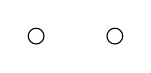
\begin{tikzpicture}
        \draw (0,0) circle (.1);
        \draw (1,0) circle (.1);
      \end{tikzpicture} \\
      \(A_2\)
      & 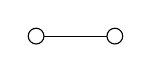
\begin{tikzpicture}
        \draw (0,0) circle (.1);
        \draw (1,0) circle (.1);
        
        \draw (0.1,0) -- (0.9,0);
                \end{tikzpicture} \\
      \(B_2\)
      &
        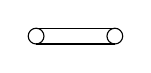
\begin{tikzpicture}
          \draw (0,0) circle (.1);
          \draw (1,0) circle (.1);

          \draw (0,0.1) -- (1,0.1);
          \draw (0,-0.1) -- (1,-0.1);
        \end{tikzpicture} \\
      \(G_2\)
      & 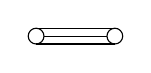
\begin{tikzpicture}
          \draw (0,0) circle (.1);
          \draw (1,0) circle (.1);

          \draw (0,0.1) -- (1,0.1);
          \draw (0.1,0) -- (0.9,0);
          \draw (0,-0.1) -- (1,-0.1);
        \end{tikzpicture} 
    \end{tabular}
  \end{center}
  For \(A_1 \times A_1\), we note that any two simple roots must be
  orthogonal, since the two \(A_1\)'s form a \(90\) degree
  angle. Thus, if \(\simpleroots = \{\alpha,\beta\}\), then \(\langle
  \alpha, \beta \rangle = 0\) and \(\langle \beta, \alpha \rangle =
  0\). So, there is no edge connecting the two vertices. \\

  In contrast, consider \(A_2\). Taking \(\simpleroots = \{\alpha,
  \beta\}\) as denoted 
  where \(A_2\) was defined, we check \[
    \langle \alpha, \beta \rangle  = 2(\alpha,\beta) = 2 \cos
    \frac{2\pi}{3} = -1 = 2 \cos(\frac{2\pi}{3}) = 2(\beta,\alpha) =
    \langle \beta, \alpha \rangle
  \]
  and thus \(\langle \alpha,\beta \rangle \langle \beta,\alpha \rangle
  = 1\). \\

  Next, consider \(B_2\) taking \(\simpleroots = \{\alpha,\beta\}\) as
  denoted where \(B_2\) was defined. We check
  \begin{align*}
    \langle \alpha,\beta \rangle
    & = 2\frac{(\alpha,\beta)}{(\beta,\beta)} = 2
      \frac{|\alpha|\sqrt{2}|\alpha| \cos \frac{3\pi}{4}}{2|\alpha|^2}
      = \sqrt{2} \cos \frac{3\pi}{4} = -1 \\
    \langle \beta,\alpha \rangle
    & = 2 \sqrt{2} \cos \frac{3\pi}{4} = -2
  \end{align*}
  Thus, \(\langle \alpha,\beta \rangle \langle \beta,\alpha \rangle =
  2\). \todo{Do \(G_2\)}
\end{example}
However, two different root systems can have the same Coxeter
graph. Luckily, with a slight fix, we can use diagrams such as these
to distinguish different root systems.
\begin{defn}
  We define the \de{Dynkin diagram} of a root system \(\roots\) to be
  the Coxeter graph with directed edges such that, given double or
  triple edges between two roots, the edges will
  point away from the longer root and towards the shorter root.
\end{defn}
We then have the following theorem.
\begin{thm}
  Up to ordering of simple roots, every Cartan matrix has a unique
  Dynkin diagram and vice versa.
\end{thm}
\begin{proof}
  \todo{Add proof or delete environment}
\end{proof}
\begin{thm}
  \(\roots\) is irreducible if and only if its Coxeter graph is
  connected. 
\end{thm}
\begin{cor}
  A root system \(\roots\) in Euclidean space \(E\) decomposes
  (uniquely) as the union of 
  irreducible root systems \(\roots_i\) (in subspaces \(E_i \subset
  E\)) such that \(E = E_1 \oplus E_2 \oplus \cdots \oplus E_k\).
\end{cor}
\section{Irreducible Root Systems}
Now that we have a structure theorem for root systems, we wish to
arrive at a classification of irreducible root systems. To do this,
one first figures out all the possible connected Coxeter graphs using
elementary geometry/graph theory. We will only summarise here.
\begin{thm}
  If \(\roots\) is an irreducible root system of rank \(\ell\), its
  Dynkin diagram is one of the following with \(\ell\) vertices:\\
  \begin{center}
    \begin{tabular}{cc}
      \(A_\ell\) with \(\ell \geq 1\)
      & 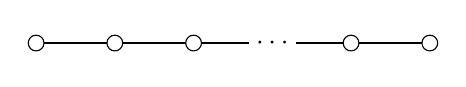
\begin{tikzpicture}
	\draw (0,0) -- (1,0);
        \draw (2,0) -- (2.7,0);
        \draw (1,0) -- (2,0);
	\draw (3.3, 0) -- (4,0);
	\draw (4,0) -- (5,0);
	
	\draw[fill=white] (0,0) circle(.1); \draw[fill=white] (1,0)
        circle(.1); \draw[fill=white] (2,0) circle(.1);
        \draw[fill=white] (4,0) circle(.1); \draw[fill=white] (5,0)
        circle(.1);
	
	\node at (3,0) {$\cdots$};
      \end{tikzpicture} \\
      \(B_\ell\) with \(\ell \geq 2\) & 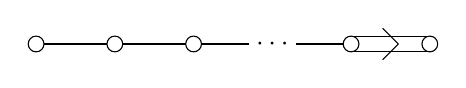
\begin{tikzpicture}

	\draw (0,0) -- (2.7,0); \draw (3.3, 0) -- (4,0); \draw (4,0.1)
        -- (5,0.1); \draw (4,-0.1) -- (5,-0.1); \draw (4.4,0.2) --
        (4.6,0); \draw (4.4,-0.2) -- (4.6,0);
		
	\draw[fill=white] (0,0) circle(.1); \draw[fill=white] (1,0)
        circle(.1); \draw[fill=white] (2,0) circle(.1);
        \draw[fill=white] (4,0) circle(.1); \draw[fill=white] (5,0)
        circle(.1);
	
	\node at (3,0) {$\cdots$};
      \end{tikzpicture} \\
      \(C_\ell\) with \(\ell \geq 3\) & 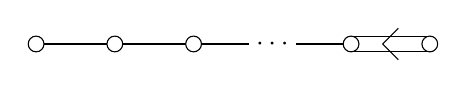
\begin{tikzpicture}

	\draw (0,0) -- (2.7,0); \draw (3.3, 0) -- (4,0); \draw (4,0.1)
        -- (5,0.1); \draw (4,-0.1) -- (5,-0.1); \draw (4.4,0) --
        (4.6,0.2); \draw (4.4,0) -- (4.6,-0.2);
		
	\draw[fill=white] (0,0) circle(.1); \draw[fill=white] (1,0)
        circle(.1); \draw[fill=white] (2,0) circle(.1);
        \draw[fill=white] (4,0) circle(.1); \draw[fill=white] (5,0)
        circle(.1);
	
	\node at (3,0) {$\cdots$};
      \end{tikzpicture}\\
      \(D_\ell\) with \(\ell \geq 4\) & \begin{tikzpicture}

	\draw (0,0) -- (2.7,0); \draw (3.3, 0) -- (4,0); \draw (4,0)
        -- (5,-.5); \draw (4,0) -- (5,.5);
	
	\draw[fill=white] (0,0) circle(.1); \draw[fill=white] (1,0)
        circle(.1); \draw[fill=white] (2,0) circle(.1);
        \draw[fill=white] (4,0) circle(.1); \draw[fill=white] (5,-.5)
        circle(.1); \draw[fill=white] (5,.5) circle(.1);
	
	\node at (3,0) {$\cdots$};
      \end{tikzpicture}\\
      \(E_6\) & \begin{tikzpicture}

	\draw (0,0) -- (4,0); \draw (2,0) -- (2,1);
	
	\draw[fill=white] (0,0) circle(.1); \draw[fill=white] (1,0)
        circle(.1); \draw[fill=white] (2,0) circle(.1);
        \draw[fill=white] (2,1) circle(.1); \draw[fill=white] (3,0)
        circle(.1); \draw[fill=white] (4,0) circle(.1);
      \end{tikzpicture}
      \\
      \(E_7\)
      & \begin{tikzpicture}

	\draw (0,0) -- (5,0); \draw (2,0) -- (2,1);
	
	\draw[fill=white] (0,0) circle(.1); \draw[fill=white] (1,0)
        circle(.1); \draw[fill=white] (2,0) circle(.1);
        \draw[fill=white] (2,1) circle(.1); \draw[fill=white] (3,0)
        circle(.1); \draw[fill=white] (4,0) circle(.1);
        \draw[fill=white] (5,0) circle(.1);
      \end{tikzpicture}
      \\
      \(E_8\)
      & \begin{tikzpicture}

	\draw (0,0) -- (6,0); \draw (2,0) -- (2,1);
	
	\draw[fill=white] (0,0) circle(.1); \draw[fill=white] (1,0)
        circle(.1); \draw[fill=white] (2,0) circle(.1);
        \draw[fill=white] (2,1) circle(.1); \draw[fill=white] (3,0)
        circle(.1); \draw[fill=white] (4,0) circle(.1);
        \draw[fill=white] (5,0) circle(.1); \draw[fill=white] (6,0)
        circle(.1);
      \end{tikzpicture}
      \\
      \(F_4\)
      & 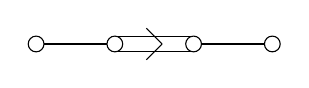
\begin{tikzpicture}

	\draw (0,0) -- (1,0); \draw (1,.1) -- (2,.1); \draw (1,-.1) --
        (2,-.1); \draw(2,0) -- (3,0); \draw (1.4,0.2) -- (1.6,0);
        \draw (1.4,-0.2) -- (1.6,0);
	
	\draw[fill=white] (0,0) circle(.1); \draw[fill=white] (1,0)
        circle(.1); \draw[fill=white] (2,0) circle(.1);
        \draw[fill=white] (3,0) circle(.1);
      \end{tikzpicture}
      \\
      \(G_2\)
      & 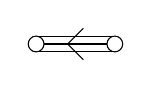
\begin{tikzpicture}

	\draw (0,0) -- (1,0); \draw (0,.1) -- (1,.1); \draw (0,-.1) --
        (1,-.1); \draw (.4,0) -- (.6,0.2); \draw (.4,0) -- (.6,-0.2);
	
	\draw[fill=white] (0,0) circle(.1); \draw[fill=white] (1,0)
        circle(.1);
      \end{tikzpicture}
    \end{tabular}
  \end{center}
  where the restrictions on \(\ell\) are to avoid duplication of
  diagrams. 
\end{thm}
\begin{proof}
  See \cite{humph}*{pp 58--63} for a full proof. In summary, we rely
  on the 
  concept of an \emph{admissible configuration} in 
  \(\R^n\), namely, a collection of unit vectors in an open half-space
  such that any two vectors form an angle of \(\frac{\pi}{2},
  \frac{2\pi}{3}, \frac{3\pi}{4}\), or \(\frac{5\pi}{6}\).
  \begin{lem}
    If \(v_1, \ldots, v_n\) form an admissible onfiguration, then they
    are linearly independent.
  \end{lem}
  \begin{lem}
    The Coxeter graph of an admissible configuration is acyclic,
    ignoring multiplicity of edgegs.  
  \end{lem}
  \begin{lem}
    Any vertex in the Coxeter graph has degree at most \(3\),
    counting multiplicity.
  \end{lem}
  \begin{lem}
    If \(v_1, \ldots, v_n\) form an admissible configuration with
    \(v_i, v_j\) connected by a single edge, then the configuration
    formed by removing \(v_i\) and \(v_j\) and replacing them with a
    single vector \(v_i+v_j\), corresponding to deleting the two nodes
    and replacing them with one in the Coxeter diagram, forms another
    admissible configuration.
  \end{lem}
  \begin{lem}
    A Coxeter graph of an admissible configuration cannot contain any
    of the following subgraphs:
    \begin{center}
      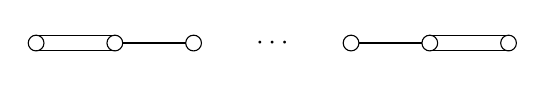
\begin{tikzpicture}
        \draw[fill=white] (0,0) circle(.1);
        \draw[fill=white] (1,0)
        circle(.1);
        \draw[fill=white] (2,0) circle(.1);
        \node at (3,0)
        {\(\cdots\)};
        \draw[fill=white] (4,0) circle(.1);
        \draw[fill=white] (5,0) circle(.1);
        \draw[fill=white] (6,0) circle(.1);

        \draw (0,0.1) -- (1,0.1);
        \draw (0,-0.1) -- (1,-0.1);
        \draw (1.1,0) -- (1.9,0);
        \draw (4.1,0) -- (4.9,0);
        \draw (5,0.1) -- (6,0.1);
        \draw (5,-0.1) -- (6,-0.1);
      \end{tikzpicture}\\
      \begin{tikzpicture}
        \draw (0,0.1) -- (1,0.1);
        \draw (0,-0.1) -- (1,-0.1);
        \draw (1,0) -- (2,0);
        \draw (4,0) -- (5,0);
        \draw (5,0) -- (6,0.5);
        \draw (5,0) -- (6,-0.5);

        \draw[fill=white] (0,0) circle(.1);
        \draw[fill=white] (1,0)
        circle(.1);
        \draw[fill=white] (2,0) circle(.1);
        \node at (3,0)
        {\(\cdots\)};
        \draw[fill=white] (4,0) circle(.1);
        \draw[fill=white] (5,0) circle(.1);
        \draw[fill=white] (6,0.5) circle(.1);
        \draw[fill=white] (6,-0.5) circle(.1);

      \end{tikzpicture}\\
      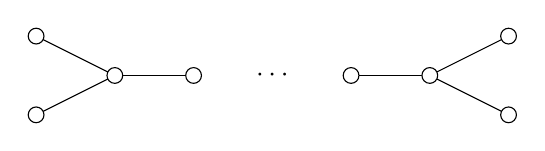
\begin{tikzpicture}
        \draw (0,0.5) -- (1,0);
        \draw (0,-0.5) -- (1,0);
        \draw (1,0) -- (2,0);
        \draw (4,0) -- (5,0);
        \draw (5,0) -- (6,0.5);
        \draw (5,0) -- (6,-0.5);

        \draw[fill=white] (0,0.5) circle(.1);
        \draw[fill=white] (0,-0.5) circle(.1);
        \draw[fill=white] (1,0)
        circle(.1);
        \draw[fill=white] (2,0) circle(.1);
        \node at (3,0)
        {\(\cdots\)};
        \draw[fill=white] (4,0) circle(.1);
        \draw[fill=white] (5,0) circle(.1);
        \draw[fill=white] (6,0.5) circle(.1);
        \draw[fill=white] (6,-0.5) circle(.1);

      \end{tikzpicture}

    \end{center}
  \end{lem}
\end{proof}
Thus, we have a complete classification of Dynkin diagrams, which
completely determines all possible Cartan matrices. Furthermore, since
we can recover a root system from its Cartan matrices, we have
effectively classified all irreducible root systems. Thus, in a sense,
root systems are a very well understood object.
\section{Automorphisms of a Root System}
As discussed before, the Weyl group is the group generated by all the
reflections across hyperplanes orthogonal to the roots of a root
system. However, this is typically only a subgroup of all automorphisms of a
root system.
\begin{lem}
  Given a root system, \(\roots\), \(\W \normsubgroup \Aut \roots\),
  that is the group of all isomorphisms of \(\roots\) onto itself.
\end{lem}
\begin{proof}
  It was left as an exercise to prove \ref{weyl-gp-conj}, that is, for \(\sigma
  \in \Aut \roots\) and \(\alpha \in \roots\), \[
    \sigma \sigma_\alpha \sigma^{-1} = \sigma_{\sigma(\alpha)}
  \]
  Thus, since the conjugate of any generator of the Weyl group is in
  the Weyl group, and \(\W \subgroup \Aut \roots\), it must be that
  \(\W \normsubgroup \Aut \roots\).
\end{proof}
Next, we define the following subgroup of \(\Aut \roots\).
\begin{defn}
  Let \(\roots\) be a root system with simple system
  \(\simpleroots\). Then, we define \[
    \Gamma := \{\sigma \in \Aut \roots \st \sigma(\simpleroots) = \simpleroots\}
  \]
\end{defn}
\begin{prop}
  Let \(\W\) be the Weyl group of a root system \(\roots\). Then, \[
    \Aut \roots \isom \W \rtimes \Gamma
  \]
\end{prop}
\begin{proof}
  Let \(\tau \in \Gamma \intersect \W\). Thus, \(\tau(\simpleroots) =
  \simpleroots\) because \(\tau \in \Gamma\). Then, by \ref{weyl-gp-and-simple-system}, since \(\tau
  \in \W\), \(\tau(\simpleroots) = \simpleroots \implies \tau =
  1\).

  Next, consider \(\tau \in \Aut \roots\). Then,
  \(\tau(\simpleroots)\) is another simple system of \(\roots\), so
  there exists a \(\sigma \in \W\) such that \(\sigma
  \tau(\simpleroots) = \simpleroots\) by \ref{weyl-gp-and-simple-system}. Thus, \(\sigma \tau \in
  \Gamma\) and \(\sigma \in \W\) together gives \(\tau \in \W
  \Gamma\). 
\end{proof}
Now, recall that for all \(\tau \in \Aut \roots\), \(\langle
\alpha,\beta \rangle = \langle \tau(\alpha), \tau(\beta) \rangle\) for
all \(\alpha, \beta \in \roots\) by definition.
\begin{prop}
  For a root system \(\roots\), every \(\tau \in \Gamma\) corresponds
  to a diagram automorphism of the Dynkin diagram associated to \(\roots\).
\end{prop}
\begin{proof}
  As noted above, for \(\tau \in \Gamma\), \(\langle
\alpha,\beta \rangle = \langle \tau(\alpha), \tau(\beta) \rangle\),
and \(\tau(\simpleroots) = \simpleroots\), so \(\tau\) will permute
the vertex labels of the Dynkin diagram while still preserving the
number of edges between them. Similarly, a diagram automorphism will
permute \(\simpleroots\) while preserving the number of edges, thus
giving an element of \(\Gamma\). Thus,
we have the desired correspondance.
\end{proof}
Thus, given that we know all the possible Dynkin diagrams, to fully
understand the automorphisms, we need only understand the Weyl group
structure of our root systems. To summarise our understanding, so far,
we have the following presentation of the Weyl group
\begin{prop}
  Let \(\roots\) be a root system with Weyl group \(\W\), simple
  system \(\simpleroots = \{\alpha_1, \ldots, \alpha_n\}\), and Cartan
  matrix \(A\). Then, \[
    \W = \left\langle \{\sigma_\alpha \st \alpha \in \simpleroots\}
      \st \sigma_\alpha^2 = 1, \text{ for }\beta \neq \pm \alpha,
    \sigma_\alpha \sigma_\beta =
      \begin{cases}
        (\sigma_\alpha \sigma_\beta)^2 = 1
        & \text{ if }\langle \alpha,\beta \rangle\langle \beta,\alpha \rangle =
        0\\
        (\sigma_\alpha \sigma_\beta)^3 = 1
        & \text{ if } \langle \alpha,\beta \rangle\langle \beta,\alpha \rangle =
        1\\
        (\sigma_\alpha \sigma_\beta)^4 = 1
        & \text{ if } \langle \alpha,\beta \rangle\langle \beta,\alpha \rangle =
        2\\
        (\sigma_\alpha \sigma_\beta)^6 = 1
        & \text{ if } \langle \alpha,\beta \rangle\langle \beta,\alpha \rangle =
        3
      \end{cases}
\right\rangle
\]
that is to say, \(\W\) is generated by reflections of the simple roots
with relations given by the Dynkin diagram of \(\roots\).
\end{prop}
\begin{proof}
  The generators come from \ref{weyl-gp-and-simple-system}. Since
  \(\alpha, \beta \in \simpleroots\), this means we can the following
  implications for \(\theta\), the angle between \(\alpha\)  and
  \(\beta\). \[
    \begin{cases}
      \langle \alpha,\beta \rangle\langle \beta,\alpha \rangle = 0
      & \implies \theta = \frac{\pi}{2} \\
      \langle \alpha,\beta \rangle\langle \beta,\alpha \rangle = 1
      & \implies \theta = \frac{2\pi}{3} \\
      \langle \alpha,\beta \rangle\langle \beta,\alpha \rangle = 2
      & \implies \theta = \frac{3\pi}{4} \\
      \langle \alpha,\beta \rangle\langle \beta,\alpha \rangle = 3
      & \implies \theta = \frac{5\pi}{6} \\
    \end{cases}
  \]
  Thus, from a geometric perspective, \(\sigma_\alpha \sigma_\beta\)
  is a rotation by \(2\theta\) on the root system. Thus, the relations
  immediately follow. 
\end{proof}
This immediately tells us the information we need to understand the
Weyl groups of irreducible root systems.
\begin{example}
  Let \(\roots = A_n\) with simple system \(\simpleroots = \{e_1-e_2,
  \ldots, e_{n-1}-e_n\}\). Then, the Weyl group generators act on the
  set \(\{e_1, \ldots, e_n\}\) by \[
    \sigma_{e_i-e_{i+1}}(e_k) = e_k -
    2\frac{(e_k,e_i-e_{i+1})}{(e_i-e_{i+1}, e_i-e_{i+1})}(e_i -
    e_{i+1}) = e_k - (\delta_{k,i}-\delta_{k,i+1})(e_i-e_{i+1})
  \]
  and so \(\sigma_{e_i-e_{i+1}}\) sends \[
    e_i \mapsto e_{i+1}, e_{i+1} \mapsto e_i, e_k \mapsto e_k \text{
      for }k \neq i,i+1
  \]
  Thus, \(f \from \W \onto \Sym_n\) via \(\sigma_{e_i-e_{i+1}} \mapsto
  (i,i+1)\), but if some \(\sigma \in \W\) has \(\sigma(e_k) = e_k\)
  for all \(k\), then \(\sigma(\simpleroots) = \simpleroots\) and thus
  \(\sigma = id\), so \(\ker f = \{id\}\) and thus \(\W \isom \Sym_n\).
\end{example}
\begin{example}
  Let \(\roots = B_n\) with simple system \(\simpleroots =
  \{e_i-e_{i+1} \st 1 \leq i \leq n-1\} \union \{e_n\}\). Then, \(\roots = \{e_i \pm e_j\} \union \{\pm
  e_i\}\). Let \(\sigma \in \W\) act on the set of pairs of vectors
  \(\{\pm e_1, \ldots, \pm e_n\}\). Then, \(\sigma\) induces a
  permutation on this set, and so we have a homomorphism \(f \from \W
  \to S_n\). Consider that \(\sigma_{e_i} \in \ker f\) since all the
  \(e_i\) are orthogonal. Furthermore, if \(\tau \in \ker f\), then,
  by the orthogonality of \(e_i\)'s, we can factor (not necessarily
  uniquely) \(\tau =
  \sigma_{e_{i_1}} \cdots \sigma_{e_{i_k}}\) \todo{I am skeptical
    about this step.}. Thus, \(\ker f = \langle
  \sigma_{e_i} \st 1 \leq i \leq n \rangle\) with all generators
  commuting. Thus, \(\ker f \isom (\Z/2\Z)^n\) and, since \(f\) must
  be surjective by virtue of the fact that we could have picked any
  short root in \(\simpleroots\) and the Weyl group acts transitively
  on the set of simple systems, we have short exact
  sequence of groups \[
    1 \to (\Z/2\Z)^n \to \W \to[f] S_n \to 1
  \]
  Furthermore, using a geometric argument, one sees that
  \(f(\sigma_{e_i-e_{i+1}}) = (i,i+1)\). From the \(A_n\) example
  above, we also know that \(\langle \sigma_{\alpha_1}, \ldots,
  \sigma_{\alpha_n} \rangle \isom S_n \subgroup \W\), so we have a
  splitting \(g \from S_n \to \W\) given by \[
    (i,i+1) \mapsto \sigma_{e_i-e_{i+1}}
  \]
  Thus, our split short exact sequence gives us \(\W \isom (\Z/2\Z)^n
  \rtimes S_n\). The \(C_n\) case is analogous by symmetry. 
\end{example}
\begin{example}
  For \(\roots = D_n = \{\pm e_i \pm e_j \st 1 \leq i,j < n, i \neq
  j\}\) with \(\simpleroots = \{e_i-e_{i+1} \st 1 \leq i \leq n-1\}
  \union \{e_{n-1}+e_n\}\), consider the action of
  \(\sigma_{e_i-e_{i+1}}\) on the set of roots. By 
  direct computation \[
    \begin{cases}
      e_i \mapsto e_{i+1} \\
      e_{i+1} \mapsto e_i \\
      e_k \mapsto e_k & k \neq i,j
    \end{cases} % \implies
    % \begin{cases}
    %   e_i\pm e_k \mapsto e_j \pm e_k\\
    %   e_j\pm e_k \mapsto e_i \pm e_k
    % \end{cases}
  \]
  and thus we have a straightforward embedding of the symmetric group
  \(S_n \into \W\) via \((i,i+1) \mapsto \sigma_{e_i-e_{i+1}}\). 
  We also compute that, for \(\sigma_{e_{n-1}+e_n}\), \[
    \begin{cases}
      e_{n-1} \mapsto -e_n \\
      e_n \mapsto -e_{n-1}
    \end{cases} % \implies
    % \begin{cases}
    %   e_i+e_j \mapsto -e_i-e_j\\
    %   e_i-e_j \mapsto e_i-e_j\\
    % \end{cases}
  \]
  Thus, \(\sigma_{e_{n-1}-e_n}\sigma_{e_{n-1}+e_n}\) will send
  \(e_{n-1} \mapsto -e_{n-1}\) and \(e_n \mapsto -e_n\). From this
  element, we are able to create elements which change (only) an even
  number of signs on the standard basis vectors of \(\R^n\) but that do not
  permute them. Because of this even-ness restriction, there can only
  be \(2^{n-1}\) such possible transformations, all of which are
  realized. Thus, looking at \(f \from \W \to S_n\) where \(f(w)\) is
  sent to the permutation \(w\) induces on the set \(\{\pm
  e_1, \ldots, \pm e_n\}\), we get (split) short exact sequence \[
    1 \to \ker f \to \W \to S_n \to 1
  \]
  where \(\ker f\) must consist of those \(2^{n-1}\) sign changing
  permutations that do not permute the basis vectors. Since these
  actions commute, we have \(\ker f \isom (\Z/2\Z)^{n-1}\) and so \(\W
  \isom (\Z/2\Z)^{n-1} \rtimes S_n\) by the splitness of the short
  exact sequence.
  % \]
  % \begin{align*}
  %   \sigma_{e_i-e_j} & \mapsto (i,j) \\
  %   \sigma_{e_i+e_j} & \mapsto (i,j)
  % \end{align*}
  % and so \(\langle \sigma_{e_i-e_j}\sigma_{e_i+e_j} \rangle \subgroup
  % \ker f\) (note that \(e_i-e_j\) and \(e_i+e_j\) are orthogonal, so
  % \(\sigma_{e_i-e_j}\) and \(\sigma_{e_i+e_j}\) commute).
\end{example}
\section{Weyl Chambers}
In understanding the geometry of root systems, we have made great use
of the set of hyperplanes orthogonal to each root. However, it is
worth considering the complement to this collection of
hyperplanes. Such a complement will be disconnected, and so we can
consider the connected components of this complement.
\begin{defn}
  Given a root system \(\roots\) of Euclidean space \(E\), we call the
  connected components of \(E \setminus \Union_{\alpha \in \roots}
  P_\alpha\) the (open) \de{Weyl chambers} of \(E\), where
  \(P_\alpha\) is the hyperplane orthogonal to 
  \(\alpha\). 
\end{defn}
\begin{example}
  In Figure \ref{fig:weyl-chamber-a2}, the root system \(A_2\) is
  drawn with 
  associated hyperplanes given by the dashed lines. Thus, there are
  \(6\) Weyl chambers. The shaded chamber above corresponds to the
  choice of simple system 
  \(\{\alpha_1,\alpha_2\}\) indicated in the figure.
  \begin{figure}
    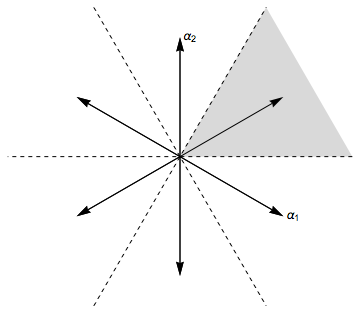
\includegraphics[scale=0.5]{images/Weyl_chambers_for_A2}
    \caption{Weyl Chambers for Root System \(A_2\) from \cite{wiki2}}
    \label{fig:weyl-chamber-a2}
  \end{figure}
\end{example}
\begin{prop}\label{weyl-chamber-props}
  Given a root system \(\roots\) of Euclidean space \(E\)
  \begin{enumerate}
  \item Each regular \(\gamma \in E\) belongs to precisely one Weyl
    chamber.
  \item Weyl chambers are in natural one-to-one correspondence with
    bases.
  \item The Weyl group acts naturally on the set of Weyl chambers, and
    this action is free and transitive.
  \end{enumerate}
\end{prop}
\begin{proof}
  Part (a) is because \(\gamma \in E\) is regular precisely when it
  does not lie in a hyperplane \(P_\alpha\). Thus, if two regular
  vectors \(\gamma, \gamma'\) are in the same Weyl chamber, they are
  both on the same sides of all the \(P_\alpha\)'s. Therefore,
  recalling the notation in the proof of \ref{regular-vec-and-base},
  \(\simpleroots(\gamma) = \simpleroots(\gamma')\). Thus, each Weyl
  chamber associates to a unique base and, furthermore, by
  \ref{regular-vec-and-base}, each base is of the form
  \(\simpleroots(z)\) for some regular \(z \in E\) which must lie in
  precisely one Weyl chamber. Thus, we have established our
  correspondance.

  For part (c), the action of the Weyl group is given by reflecting
  the Weyl chamber across the appropriate hyperplane. The transitivity
  and free-ness
  of this action comes from the correspondance with a choice of base
  along with theorem \ref{weyl-gp-and-simple-system}.
\end{proof}
\begin{defn}
  Given a choice of \(\simpleroots\), we call the Weyl chamber
  corresponding to this choice consisting of all \(v \in E\) such that
  \((v,\alpha) > 0\) for all \(\alpha \in \simpleroots\) the
  \de{fundamental Weyl chamber relative to \(\simpleroots\)}.
  Geometrically, this says that the fundamental Weyl chamber consists
  of those vectors forming an acute angle with all of the simple roots.
\end{defn}
At first glance, it is not apparent what value the Weyl chamber
perspective gives over the choice of base persepctive, but there are
some useful techniques that use closure arguments, such as
\begin{thm}\label{weyl-chamber-closure-contains-one-point-in-orbit}
  Fix a Weyl chamber \(C\). Then, for all \(v \in E\), the Weyl group
  orbit of \(v\) contains exactly one point in the closure \(\ov{C}\)
  of \(C\).
\end{thm}
\begin{proof}
  Consider the closure \(\ov{C}\) of \(C\). By construction, every
  vector \(v \in E\) must lie in the closure of some chamber and, by
  \ref{weyl-chamber-props}(c), \(\W\) acts transitively on the
  chambers. Thus, each orbit 
  of \(\W\) on \(V\) intersects \(\ov{C}\). \\

  Now, let \(v_1, v_2 \in \ov{C}\) with \(w(v_1) = v_2\) for some \(w
  \in \W\). If \(\ell(w)
  = 0\), then \(w = 1\) and so \(v_1 = v_2\). Now, let us proceed by
  assuming that, if \(v_1, v_2 \in \ov{C}\) and \(w(v_1) = v_2\) for
  some \(w \in \W\) with \(\ell(w) < n\), then \(v_1 = v_2\). Then, if
  \(w(v_1) = v_2\) for \(\ell(w) = n\), we know there is at least one
  \(\alpha_i \in \simpleroots\) such that \(w(\alpha_i) \in
  \roots^-\). Therefore, we have \[
    0 \leq \langle v_1, \alpha_i \rangle = \langle v_2, w(\alpha_i)
    \rangle \leq 0 \implies \langle v_i, \alpha_i \rangle = 0
  \]
  Therefore, \(\sigma_{\alpha_i}(v_1) = v_1\) and thus \(w
  \sigma_{\alpha_i}(v_1) = v_2\). However, the only positive root that
  becomes negative under the action of \(\sigma_{\alpha_i}\) is
  \(\alpha_i\). Therefore, the positive roots made negative by \(w\)
  and \(w\sigma_{\alpha_i}\) are the same except for \(\alpha_i\),
  which is made negative only by \(w\). Therefore, \[
    \ell(w) = \ell(w s_{\alpha_i})+1 \implies \ell(w s_{\alpha_i}) =
    \ell(w) - 1
  \]
  and so \(v_1 = v_2\) by the inductive hypothesis.
\end{proof}
An immediate consequence of the second part of this proof is the
following
\begin{lem}\label{lem-10-3-B}
  \cite{humph}*{Lemma 10.3B p 52} If \(v_1,v_2 \in \ov{C}\) such that
  \(w(v_1) = v_2\) for some \(w \in \W\), then \(w\) is a product of
  simple reflections which fix \(v_1\). In particular, \(v_1 = v_2\).
\end{lem}
\section{Weights}
Let $\weightlattice$ be a collection of vectors $\lambda \in E$ such that
$\langle \lambda, \alpha \rangle \in \Z$ for all $\alpha \in
\roots$. We call the elements
of $\weightlattice$ \de{weights}. We note that 
$\weightlattice$ is endowed with a subgroup structure with vector addition as
the operation since $\langle
\lambda_1+\lambda_2, \alpha \rangle = \langle \lambda_1, \alpha
\rangle + \langle \lambda_2, \alpha \rangle$.
\begin{defn}
  We say the \de{root lattice} is the subgroup of $\weightlattice$ generated
  by $\roots$. We denote this $\rootlattice$. 
\end{defn}
Note that $\rootlattice$ is actually a lattice since it is a $\Z$-span of
a basis of $E$.
\begin{defn}
  Fix a base $\simpleroots \subset \roots$. We say that $\lambda \in \weightlattice$
  is \de{dominant} if all the integers $\langle \lambda, \alpha
  \rangle$ are nonnegative for all $\alpha \in \simpleroots$. If they are
  all positive, then $\lambda$ is \de{strongly dominant}.
\end{defn}
We denote by $\weightlattice^+$ the set of all dominant weights.
\begin{defn}
  Let $\simpleroots = \{\alpha_1, \ldots, \alpha_n\}$. Then, we know that
  $\{\alpha_1^\vee, \ldots, \alpha_n^\vee\}$ forms a basis of
  $E$. Then, if we have the dual basis to this basis, $\{\omega_1,
  \ldots, \omega_n\}$, we can check that the $\omega_i$ are all
  dominant weights which we will call the \de{fundamental dominant
    weights (relative to $\simpleroots$)}. In otherwords, the
  fundamental dominant weights are such that \(\langle \omega_i,
  \alpha_j \rangle = \delta_{i,j}\). \todo{Check this definition with
    the coroots.}
\end{defn}
\begin{defn}
  We say that $\weightlattice/\rootlattice$ is the \de{fundamental group} of
  $\roots$. 
\end{defn}
To see that $\weightlattice/\rootlattice$ is a finite group, we can  view both
$\weightlattice$ and $\rootlattice$ as $\Z$-modules. Then, $\weightlattice \isom \Z^m$
where $m$ is the dimension of $\weightlattice$. By definition, $\rootlattice$ is a
submodule of $\weightlattice$ but has the same dimension. Both are 
free. So, the quotient will be some finite group. More concretely, one
notes that the Cartan matrix is a change of basis matrix, so to write
the \(\omega_i\) in terms of the \(\alpha_i\), we can invert the
Cartan matrix. Thus,
\begin{prop}
  Given Cartan matrix \(M\) of a root system \(\roots\),
  \begin{enumerate}
  \item The transpose of the Cartan matrix expresses the simple roots
    as linear combinations of the fundamental weights.
  \item The index of
  \(\rootlattice\) in \(\weightlattice\) is given by \(\det C\).
  \end{enumerate}
\end{prop}
\begin{proof}
  Write \(\alpha_i = \sum_j c_{i,j} \omega_j\) for \(c_{i,j} \in
  \Z\). Then, we see
  \begin{equation}
    \label{eq:weight-decomp}
    M_{i,k} = \langle \alpha_i, \alpha_k \rangle = \sum_{j} c_{i,j}
    \langle 
    \omega_j, \alpha_k \rangle = c_{i,k}
  \end{equation}
  giving us \[
    \alpha_i = \sum_j c_{i,j} \omega_j =
    \sum_j M_{i,j} \omega_j
  \]
  Thus, the Cartan matrix is a change of basis matrix to write the
  \(\alpha_i\)'s in terms of the \(\omega_i\)'s. To go the other
  direction, we simply invert \(M\), which is a matrix with entries in
  \(\Z\), so \(M^{-1} = \frac{1}{\det M} \operatorname{adj}(M)\), and
  thus \(\det M \cdot \omega_i \in \rootlattice\).
\end{proof}
\begin{example}
  Consider the root system \(A_2\) with \(\simpleroots =
  \{\alpha,\beta\}\). Then, since the Cartan matrix is \[
    M = \left(
      \begin{array}{cc}
        2&-1\\
        -1&2
      \end{array}
\right)
  \]
  We have \[
    \begin{cases}
      \alpha & = 2 \omega_1 - \omega_2\\
      \beta & = -\omega_1 + 2 \omega_2
    \end{cases}
    \implies
    \begin{cases}
      \omega_1 & = \frac{2}{3} \alpha + \frac{1}{3} \beta\\
      \omega_2 & = \frac{1}{3} \alpha + \frac{2}{3} \beta
    \end{cases}
  \]
\end{example}
\todo{Compute the index for each type.}
Recall the
partial order on roots \ref{partial-order-on-roots}. We can extend
this to a partial order on weights as follows.
\begin{defn}
  Given \(\lambda,\mu \in \weightlattice\), we say \(\mu \prec
  \lambda\) if and only if \(\lambda-\mu\) is a sum of positive roots.
\end{defn}
In some ways, dominant weights serve as a good notion for a base of
the weights, by virtue of the following proposition.
\begin{prop}\label{weight-is-conj-to-unique-dominant-weight}
  \cite{humph}*{p 68} Each weight is conjugate under \(\W\) to one and
  only one dominant weight. If \(\lambda\) is dominant, then \(w
  \lambda \prec \lambda\) for all \(w \in \W\), and if
  \(\lambda\) is strongly dominant, then \(w \lambda = \lambda\)
  only when \(w = 1\).
\end{prop}
\begin{proof}
  This result follows from
  \ref{weyl-chamber-closure-contains-one-point-in-orbit} and
  \ref{lem-10-3-B} since all the fundamental weights lie in the
  closure of the fundamental Weyl chamber.
\end{proof}
However, dominant weights are not not necessarily maximal with respect
to the partial order in general.
\begin{example}
  Consider the weight lattice for \(A_2\) with
  \(\simpleroots=\{\alpha,\beta\}\), the standard choice. Then,
  \(\lambda = 3\alpha+\beta\) has \[
    \langle \lambda, \beta \rangle = -3+2 = -1
  \]
  so \(\lambda\) is not a dominant weight. However, \(\lambda-\alpha\)
  has \[
    \langle \lambda-\alpha, \beta \rangle = -2+2=0, \ \ \langle
    \lambda-\alpha, \alpha \rangle = 4-1 = 3
  \]
  and thus is a dominant weight. Therefore, \(\lambda-\alpha \prec
  \lambda\) since \(\lambda - (\lambda-\alpha) = \alpha \in
  \simpleroots\), but \(\lambda\) is not dominant.
\end{example}
However, given a fixed dominant weight, the space of all such examples
is finite.
\begin{lem}\label{finite-num-of-misbehaved-weights}
  \cite{humph}*{p 70} Let \(\lambda\) be a dominant weight. Then, the
  number of dominant 
  weights \(\mu\) such that \(\mu \prec \lambda\) is finite.
\end{lem}
\begin{proof}
  Observe that, since \(\lambda-\mu\) is a sum of positive roots, \[
    0 \leq (\lambda+\mu, \lambda-\mu) = (\lambda,\lambda)-(\mu,\mu)
  \]
  so \(\mu \in \{x \in E \st (x,x) \leq (\lambda,\lambda)\}\), which
  is compact. Furthermore, the dominant weights is a discrete set, so
  there can only be a finite number of such \(\mu\).
\end{proof}
\begin{prop}
  \cite{humph}*{p 70} Recall \(\displaystyle \halfsum = \frac{1}{2} \sum_{\alpha \in \roots, \alpha \succ
    0} \alpha\) (\ref{half-sum-defn}). As discussed before, \(\halfsum
  \in \weightlattice\). Furthermore,
  \begin{enumerate}
  \item \(\halfsum\) is a (strongly) dominant weight and, in fact, \[
      \halfsum = \sum_{i=1}^n \omega_i
    \]
  \item For \(\mu \in \weightlattice^+\) and \(\nu = w^{-1}(\mu)\) for
    \(w \in \W\) we have \[
      (\nu+\halfsum,\nu+\halfsum) \leq (\mu+\halfsum, \mu+\halfsum)
    \] with equality only if
    \(\nu=\mu\). 
  \end{enumerate}
\end{prop}
\begin{proof}
  For (a), observe \[
    \sigma_i \halfsum = \halfsum-\alpha_i \implies (\halfsum-\alpha_i,
    \alpha_i) = (\sigma_i^2 \halfsum, \sigma_i \alpha_i) = (\halfsum,
    -\alpha_i) \implies 2(\halfsum, \alpha_i) = (\alpha_i,\alpha_i) = 2
  \]
  Thus, \(\langle \halfsum, \alpha_i \rangle = 1\), so \[
    \halfsum \overset{\ref{eq:weight-decomp}}{=} \sum_i \langle \halfsum, \alpha_i \rangle \omega_i =
    \sum_i \omega_i
  \]
  For (b), observe
  \begin{align*}
    (\nu+\halfsum,\nu+\halfsum)
    & = (w(\nu+\halfsum), w(\nu+\halfsum)) \\
    & = (\mu+w\halfsum, \mu+w\halfsum) \\
    & = (\mu + \halfsum, \mu + \halfsum) - 2(\mu, \halfsum-w\halfsum)
    \\
    & \leq (\mu+\halfsum, \mu+\halfsum)
      & \text{ since }\mu \in \weightlattice^+ \text{ and } \halfsum -
        w\halfsum \text{ is a sum of positive roots}
  \end{align*}
  with equality only if \((\mu, \halfsum-w\halfsum) = 0\) by
  \ref{weight-is-conj-to-unique-dominant-weight}. \todo{Why is the last
    equality true?} However, this gives us \[
    (\mu,\halfsum) = (\mu, w\halfsum) = (\nu, \halfsum) \implies
    (\mu-\nu,\halfsum) = 0
  \]
  but \(\mu-\nu\) is a sum of positive roots and \(\halfsum\) is
  strongly dominant, so it must be that \(\mu=\nu\).
\end{proof}
Finally, we give a discussion of the notion of saturated sets of
weights. This idea is important for those interested in understanding
how \cite{humph} proves results on irreducible finite dimensional
semisimple Lie
algebra representations over an algebraically closed field of
characteristic \(0\) in section \(21\).
\begin{defn}
  We call a subset \(S \subset \weightlattice\) \de{saturated} if, for
  all \(\lambda \in S\), \(\alpha \in \roots\), and \(i\) between
  \(0\) and \(\langle \lambda, \alpha \rangle\), the weight
  \(\lambda-i \alpha \in S\). We say a saturated set of weights has a
  \de{highest weight} \(\lambda\) if \(\lambda \in S\) and \(\mu \prec
  \lambda\) for all \(\mu \in S\).
\end{defn}
\begin{prop}
  Given a saturated set of weights \(S\), we have the following
  \begin{enumerate}
  \item \(S\) is stable under \(\W\), that is, \(\sigma_\alpha \lambda
    = \lambda - \langle \lambda, \alpha \rangle \alpha
    \in S\) for all \(\lambda \in S, \alpha \in \roots\).
  \item If \(S\) has a highest weight, then \(S\) must be finite.
  \item If \(S\) has highest weight \(\lambda\), then if \(\mu \in
    \weightlattice^+\) and \(\mu \prec \lambda\), then \(\mu \in S\).
  \item (Optional) If \(S\) has highest weight \(\lambda\), then if
    \(\mu \in 
    S\), then \[
      (\mu+\halfsum, \mu+\halfsum) \leq (\lambda + \halfsum, \lambda +
      \halfsum)
    \]
    with equality only if \(\mu = \lambda\).
  \end{enumerate}
\end{prop}
\begin{proof}
  Part (a) is immediate from the definition of \(S\) being
  saturated. For part (b), we note that the number of dominant weights
  less than the highest weight, say \(\lambda \in S\), must be
  finite by \ref{finite-num-of-misbehaved-weights}. Thus, since our
  root system is also finite, each dominant weight will only have a
  finite number of other weights to make \(S\) saturated. \\

  For (c), we take an arbitrary \(\mu' = \mu+\sum_{\alpha \in
    \simpleroots} k_\alpha \alpha \in S\) with \(k_\alpha \in
  \Z^+\). One reduces one of the \(k_\alpha\) while still remaining in
  \(S\) until only \(\mu \in S\). \\

  For (d), we can reduce to \(\mu\) being dominant using part (c). If
  \(\mu = \lambda - \pi\) for \(\pi\) a sum of positive roots, we have
  \begin{align*}
    (\lambda+\halfsum, \lambda+\halfsum) - (\mu+\halfsum,
    \mu+\halfsum)
    & = (\lambda + \halfsum, \lambda+\halfsum) -
      (\lambda+\halfsum-\pi, \lambda+\halfsum-\pi) \\
    & = (\lambda+\halfsum, \pi)+(\pi, \mu+\halfsum) \\
    & \geq (\lambda+\halfsum, \pi) \\
    & \geq 0
  \end{align*}
  where the inequalities follow because \(\mu+\halfsum\) and
  \(\lambda+\halfsum\) are dominant. Because \(\lambda+\halfsum\) is
  strongly dominant, equality holds only if \(\pi = 0\).
\end{proof}
The proposition above gives us a good picture of what a saturated set
of weights \(S\) looks like if it has a highest weight. Namely, \(S\)
consists of all dominant weights lower than or equal to highest weight
\(\lambda\) and the conjugates of all these weights under \(\W\)
\begin{cor}
  \cite{humph}*{p 71} Given \(\lambda \in \weightlattice^+\), there exists precisely one
  set of saturated weights \(S\) such that \(\lambda\) is a highest
  weight of \(S\).
\end{cor}
\begin{proof}
  Given the exposition above, for \(\lambda \in \weightlattice^+\), we
  see that at most one saturated set of weights can exist with
  \(\lambda\) the highest weight. Conversely, given \(\lambda \in
  \weightlattice^+\), let us construct a saturated set of weights where
  \(\lambda\) is a highest weight.
  \begin{enumerate}
  \item Take \(S\) to be the set of all dominant weights below
    \(\lambda\) and their \(\W\)-conjugates.
  \item Observe that \(S\) is stable under the \(\W\). Then, \(w \mu
    \prec \mu\) for all dominant weights \(\mu\) and all \(w \in
    \W\) by \ref{weight-is-conj-to-unique-dominant-weight}. Thus, \[
      S = \{\mu \in \weightlattice \st w \mu \prec \lambda \text{ for
        all } w \in \W\}
    \]
    Take \(\alpha \in \roots\). For \(\mu' = \mu - k \alpha\) for
    \(k\) between \(0\) and 
    \(\langle \mu, \alpha \rangle\), we wish to show \(\mu' \in S\).
  \item Since \(\mu'\) is on the \(\alpha\)-chain of \(\mu\),
    \(w(\mu')\) is on the \(w(\alpha)\)-chain from \(w(\mu)\) to
    \(w(\mu-\langle \mu,\alpha \rangle \alpha) = w(\mu)-\langle
    \mu,\alpha \rangle w(\alpha)\). Thus, we have \[
      w \mu \prec w \mu' \prec w \mu - \langle \mu,\alpha \rangle w
      (\alpha) \text{ or } w \mu - \langle \mu,\alpha \rangle w
      (\alpha) \prec w \mu' \prec w\mu
    \]
  \item Note, howver, \(w\mu\) and \(w \mu - \langle \mu,\alpha \rangle w
      (\alpha)\) are both in the \(\W\)-orbit of \(\mu\), so by the
      description of \(S\) above, they are both lower than
      \(\lambda\). Therefore, \(w \mu' \prec \lambda\) for all \(w \in
      \W\), thus giving us \(\mu' \in S\) by our description of \(S\).
  \end{enumerate}
\end{proof}
\section{Appendix: Summary Information}
Throughout, we denote \(\epsilon_i\) for the \(i\)th standard basis
vector of \(\R^n\). Refer to Section \ref{standard-examples} for definitions of these root systems.
\subsection{Type \(A_n\)}
\begin{prop}
The root system \(A_n \subset \R^{n+1}\) has
\begin{enumerate}
\item \(\roots = \{\epsilon_i - \epsilon_j \st 1 \leq i \neq j \leq
  n+1\}\) and \(|\roots| = n(n+1)\).
\item The canonical choice of simple roots is \[
    \simpleroots = \{\epsilon_i - \epsilon_{i+1} \st 1 \leq i < n+1\}
  \]
  and thus \(\roots^+ = \{\epsilon_i-\epsilon_j \st 1 \leq i < j \leq
  n+1\}\).
\item From the action on \(\{e_1, \ldots, e_n\}\), one can infer
  \(\W = \Sym_n\). 
\item The fundamental weights are given by \(\omega_i =
  \epsilon_1+\cdots+\epsilon_i\) for \(1 \leq i \leq n\) and \[
    \halfsum = n \epsilon_1 + (n-1) \epsilon_2 + \cdots + \epsilon_n
  \]
\end{enumerate}
\end{prop}
\subsection{Type \(B_n\)}
\begin{prop}
  The root system \(B_n \subset \R^n\) has
  \begin{enumerate}
  \item \(\roots = \{\pm(\epsilon_i + \epsilon_j) \st 1 \leq i < j
    \leq n\} \union \{\pm (\epsilon_i - \epsilon_j) \st 1 \leq i < j
    \leq n\} \union \{\pm \epsilon_i \st 1 \leq i \leq n\}\) and so
    \(|\roots| = 2n(n-1)+2n = 2n^2\).
  \item The canonical choice of simple roots is \[
      \simpleroots = \{\epsilon_i - \epsilon_{i+1} \st 1 \leq  i < n\}
      \union \{\epsilon_n\}
    \]
    and thus \(\roots^+ = \{\epsilon_i+\epsilon_j \st 1 \leq i < j
    \leq n\} \union \{\epsilon_i-\epsilon_j \st 1 \leq i < j
    \leq n\} \union \{\epsilon_i \st 1 \leq i \leq n\}\).
  \item Since the Dynkin diagram has no graph automorphisms, it must
    be that \(\W = \Aut \roots\). Furthermore, automorphisms can
    permute \(\{\epsilon_1, \ldots, \epsilon_n\}\) and change any of
    the signs, thus giving \(\W = (\Z/2)^n \rtimes \Sym_n\).
  \item The fundamental weights are given by \[
      \omega_i = \epsilon_1 + \cdots + \epsilon_i, (i < n) \ \ \omega_n
      = \frac{1}{2}(\epsilon_1 + \cdots + \epsilon_n)
    \]
    and \[
      \halfsum = \frac{1}{2}((2n-1)\epsilon_1 + (2n-3)\epsilon_2 +
      \cdots + \epsilon_n)
    \]
  \end{enumerate}
\end{prop}
\subsection{Type \(C_n\)}
\begin{prop}
  The root system \(C_n \subset \R^n\) has
  \begin{enumerate}
  \item \(\roots = \{\pm(\epsilon_i+\epsilon_j) \st 1 \leq i < j \leq
    n\} \union \{\pm(\epsilon_i - \epsilon_j) \st 1 \leq i < j
    \leq n\} \union \{\pm 2 \epsilon_i\}\) and so \(|\roots| =
    2n(n-1)+2n = 2n^2\) just as in \(B_n\).
  \item The canonical choice of simple roots is \[
      \simpleroots = \{\epsilon_i - \epsilon_{i+1} \st 1 \leq i < n\}
      \union \{2 \epsilon_n\}
    \]
    and thus \(\roots^+ = \{\epsilon_i+\epsilon_j \st 1 \leq i < j
    \leq n\} \union \{\epsilon_i-\epsilon_j \st 1 \leq i < j
    \leq n\} \union \{2 \epsilon_i \st 1 \leq i \leq n\}\).
  \item \(C_n\) presents a somewhat dual situation to \(B_n\) and thus
    also has Weyl group \(\W = (\Z/2)^n \rtimes \Sym_n\).
  \item The fundamental weights are given by \[
      \omega_i = \epsilon_1 + \cdots + \epsilon_i, (i \leq n)
    \]
    and \[
      \halfsum = n \epsilon_1 + (n-1) \epsilon_2 + \cdots + \epsilon_n
    \]
  \end{enumerate}
\end{prop}
\subsection{Type \(D_n\)}
\begin{prop}
  The root system \(D_n \subset \R^n\) has
  \begin{enumerate}
  \item \(\roots = \{\epsilon_i - \epsilon_j \st 1 \leq i \neq j
    \leq n\} \union \{\pm(\epsilon_i + \epsilon_j) \st 1 \leq i < j
    \leq n\}\) and so \(|\roots| = n(n-1)+2\frac{n(n-1)}{2} =
    2n(n-1)\).
  \item The canonical choice of simple roots is \[
      \simpleroots = \{\epsilon_i - \epsilon_{i+1} \st 1 \leq i < n\}
      \union \{\epsilon_{n-1}+\epsilon_{n}\}
    \]
    and thus \(\roots^+ = \{\epsilon_i \pm \epsilon_j \st 1 \leq i < j
    \leq n\}\).
  \item \(D_n\) has Weyl group \(\W = (\Z/2)^{n-1} \rtimes \Sym_n\).
  \item The fundamental weights are given by \[
      \begin{cases}
        \omega_i = \epsilon_1 + \cdots + \epsilon_i & i < n-1\\
        \omega_{n-1} = \frac{1}{2}(\epsilon_1 + \cdots +
        \epsilon_{n-1} - \epsilon_n) \\
        \omega_n = \frac{1}{2}(\epsilon_1 + \cdots +
        \epsilon_{n-1}+\epsilon_n) 
      \end{cases}
    \]
    and thus \[
      \halfsum = (n-1) \epsilon_1 + (n-2) \epsilon_2 + \cdots +
      \epsilon_{n-1} 
    \]
  \end{enumerate}

\end{prop}

\begin{bibdiv}
  \begin{biblist}
    \bib{humph}{book}{
      author={Humphreys, James E.}
      title={Introduction to Lie Algebras and Representaton Theory}
      year={1972}
      note={Third printing, revised}
    }
    \bib{cat-o}{book}{
      author={Humphreys, James E.}
      title={Representations of Semisimple Lie Algebras in the BGG
        Category $\mathcal{O}$}
      year={2008}
    }
    \bib{wiki}{misc}{
      author={Wikipedia}
      title={Root system --- Wikipedia{,} The Free Encyclopedia}
      year={2017}
      note={[Online; accessed 21-February-2017] \url{https://en.wikipedia.org/w/index.php?title=Root_system&oldid=759729605}}
    }
    \bib{wiki2}{webpage}{
      author={Wikipedia}
      author={Mathphysman-Mathematica}
      title={The shaded region is the funamental Weyl chamber for the
        base}
      year={2018}
      note={[Online; accessed 7-March-2018] \url{https://en.wikipedia.org/wiki/Weyl_group\#/media/File:Weyl_chambers_for_A2.png}}
    }
  \end{biblist}
\end{bibdiv}

\end{document}
%%% Local Variables:
%%% mode: latex
%%% TeX-master: t
%%% End:
